% Idea general

% \begin{itemize}
%     \item Parser C3D
%     \item Entorno Bevy
%     \item creación configuraciones (toml)
% \end{itemize}


\chapter{Desarrollo del proyecto} \label{sec:cap3}

Este proyecto se ha llevado a cabo en diferentes etapas, añadiendo mejoras progresivamente. Este capítulo explica cómo, partiendo de un entorno simple creado con \textit{Bevy}, se ha ido añadiendo funcionalidad hasta llegar a un entorno tridimensional completo, capaz de representar cualquier movimiento, así como trazas, vectores y uniones entre marcadores, con numerosas opciones de personalización.

Este capítulo muestra ejemplos del desarrollo del proyecto, utilizando un fichero \ac{C3D} de ejemplo. Este fichero ha sido capturado por las cámaras de INEF, que representa un swing de golf, y ha sido capturado con el sistema de la marca Vicon explicado en el \autoref{sec:cap2}. Como características técnicas, se trata de una grabación a 240 \ac{Hz}, tomado con 6 cámaras, y con un total de 585 marcadores, de los cuales 291 son marcadores de posición, y los restantes simbolizan aceleraciones, velocidades y fuerzas.

Este capítulo comienza explicando la estructura del proyecto, introduciendo así los diferentes módulos que lo componen. A continuación, se explica la integración del \textit{parser} de \ac{C3D} en el proyecto, y cómo se ha modificado para adaptarlo a las necesidades del mismo. Después, se explica la integración de \textit{Bevy}, y finalmente, se explica la carga de ficheros y la configuración del programa, que diferencian a este proyecto al aportar numerosas opciones de personalización.


\section{Estructura del proyecto} \label{sec:estructura-programa}

Siguiendo un principio modular, el proyecto se ha implementado en diferentes módulos, cada uno de los cuales forma un \textit{plugin}, que se integran en el módulo principal. Estos módulos son independientes entre sí, y cada uno de ellos tiene una función específica. De este modo, se consigue un código más limpio y fácil de mantener.

La estructura general consta de un módulo principal, que se encarga de la representación de la información proporcionada por cada uno de los módulos secundarios. Estos módulos secundarios se encargan de cada una de las funciones específicas del programa, como la carga de ficheros \ac{C3D} y ficheros de configuración y la implementación de una interfaz gráfica. Además, existe un módulo específico para la carga de ficheros en entornos web, eliminando las restricciones de los navegadores en cuanto a la carga de ficheros.

Los módulos que se han implementado son los siguientes:

\begin{itemize}
    \item \textbf{\texttt{app\_control}:} Es el módulo principal del programa. Se encarga de la orquestación de los diferentes módulos, inicialización de recursos\footnote{Un recurso es una estructura de datos que se utiliza para almacenar información en el programa \autocite{Resources,ResourcesUnofficialBevy}.} y generación del entorno. A su vez, está compuesto por diferentes submódulos, que son:
    \begin{itemize}
        \item \texttt{file\_drop}: Se encarga de gestionar la carga de ficheros \ac{C3D} y de configuración y de la creación de los eventos necesarios para la representación del \ac{C3D} en el entorno 3D.
        \item \texttt{markers}: Se encarga de la representación de los marcadores en el entorno 3D, incluyendo su generación, actualización y eliminación.
        \item \texttt{joins}: Se encarga de la representación de las uniones entre los marcadores en el entorno 3D, incluyendo su generación, actualización y eliminación. 
        \item \texttt{traces}: Se encarga de la representación de las trazas de los marcadores en el entorno 3D, incluyendo su generación, actualización y eliminación.
        \item \texttt{vectors}: Se encarga de la representación de los vectores en el entorno 3D, incluyendo su generación, actualización y eliminación.
        \item \texttt{mouse\_keyboard}: Se encarga de la gestión de los eventos del ratón y el teclado, así como del manejo de la cámara.
    \end{itemize}
    \item \textbf{\texttt{bevy\_c3d\_mod}:} Es una modificación del \textit{crate} \textit{bevy\_c3d} \autocite{BiomechanicsfoundationBevy_c3d2024}. Se encarga de la lectura y generación de los \textit{assets} necesarios para la representación del \ac{C3D} en el entorno 3D. 
    \item \textbf{\texttt{c3d\_config}:} Este módulo se encarga de la lectura del fichero de configuración y de la generación de los \textit{assets} necesarios para la carga del fichero de configuración, integrándose con el entorno de \textit{Bevy}.
    \item \textbf{\texttt{gui}:} Este módulo se encarga de la generación de la interfaz gráfica en dos dimensiones, es decir, es un conjunto de paneles, botones y gráficos que se usan para interactuar con el entorno 3D. A su vez, este módulo se divide en diferentes submódulos, que son:
    \begin{itemize}
        \item \texttt{metric\_dashboard}: Se encarga de la generación de una ventana flotante que permite obtener diferentes métricas.
        \item \texttt{milestones}: Se encarga de la lectura, representación y navegación a través de los eventos del \ac{C3D}.
        \item \texttt{theme}: Genera un un botón para variar entre un fondo claro y oscuro en el entorno 3D. Este botón permite mejorar el contraste entre el fondo y los marcadores, y por tanto, mejorar la visibilidad de los mismos. Además, interactúa con el motor de \textit{Bevy} para capturar las cámaras y realiza este cambio de manera autónoma.
    \end{itemize}
    \item \textbf{\texttt{web\_bevy\_blob\_loader}:} Este módulo se basa en el \textit{crate} \textit{web\_bevy\_blob\_loader} \autocite{kayhKayhhhBevy_web_file_drop2024}, y lo modifica para adaptarlo a la última versión de \textit{Bevy}. Para ello, se ha modificado su dependencia a \textit{bevy\_blob\_loader} \autocite{kayhKayhhhBevy_blob_loader2024}, realizando una adaptación a la última versión de \textit{Bevy}.
\end{itemize}

Además de los módulos ya mencionados, se ha modificado el \textit{crate} \texttt{c3dio}, como se explica en \autoref{sec:parser-c3d}.

\section{Analizador de ficheros \acs{C3D}} \label{sec:parser-c3d}
Un fichero \ac{C3D} se debe integrar con el resto del programa. Para ello, se debe contar con un analizador (comúnmente llamado \textit{parser}) que trate con el binario, que es un módulo secundario del proyecto, especializado en la traducción del formato \ac{C3D} a una estructura de datos interna que se integre con el resto del código.

Se ha partido del \textit{crate}\footnote{Como se explica en el \autoref{apx:herramientas_usadas}, un \textit{crate} es una unidad mínima de compilación de Rust. En este caso, un \textit{crate} representa una biblioteca creada para analizar los ficheros \ac{C3D}.} de \textit{Rust} \texttt{bevy-c3d}. Este \textit{crate} depende a su vez del \textit{crate} \texttt{c3dio}, que es un analizador para ficheros \ac{C3D}, pero integrado a \textit{Bevy}. De este modo, se consigue un \textit{Asset} que se puede cargar en el motor de juego.

Se ha modificado el \textit{crate} \texttt{c3dio} para adaptarlo a las necesidades del proyecto. En este caso, se han arreglado dos errores graves que impiden la compatibilidad con los ficheros generados por Vicon. Ambos errores se deben a modificaciones en la especificación introducidos de manera unilateral por Vicon. El primero de ellos se debe a una modificación en la especificación que cambia la manera de codificar los eventos, que hace que no se lea ningún evento del \ac{C3D}. El segundo error se debe a que Vicon elimina una restricción de la especificación, que limita el número de marcadores a 255. En este caso, Vicon permite un número ilimitado de marcadores, lo que provoca que el \textit{parser} solo reconozca los primeros 255 marcadores, y el resto no se lean.   

\section{Integración de \textit{Bevy} en el proyecto} \label{sec:bevy}

Este proyecto usa el motor de videojuegos \textit{Bevy} como base para generar un entorno tridimensional donde representar el \ac{C3D}. Bevy sigue el paradigma \ac{ECS}, separando entre entidades, componentes y sistemas. Las entidades son los objetos que se representan en el entorno tridimensional, los componentes son las propiedades de estas entidades, y los sistemas son las funciones que se aplican a estas entidades. Este paradigma permite una gran flexibilidad y escalabilidad, lo que lo hace ideal para este tipo de proyectos \autocite{prdevingDeepdivingEntityComponent2023}.

Se muestra en la \autoref{fig:entorno3D} una imagen del entorno tridimensional creado con \textit{Bevy}, antes de cargar el fichero de datos en formato \ac{C3D}.


\begin{figure}[H]
  \centering
  \includegraphics[width=\textwidth]{imagenes/entorno3D.png}
  \caption{Entorno 3D creado con Bevy (modo oscuro)}
  \label{fig:entorno3D}
\end{figure}

En este entorno destacan el plano central, representado en un color verde oscuro, y, apoyándose sobre él, 3 vectores que sirven como referencia. El código que genera estos vectores se explica en el \autoref{apx:spawn_ref_vec}, demostrando la flexibilidad de \textit{Bevy} y el potencial de Rust. 

El pequeño botón que aparece en la esquina superior izquierda permite cambiar el color de fondo, alternando entre un modo claro y un modo oscuro. En la \autoref{fig:modo_claro} se muestra el entorno en modo claro. Variar entre estos modos permite mejorar el contraste con los marcadores, y por tanto, mejorar la visibilidad de los mismos.

\begin{figure}[H]
  \centering
  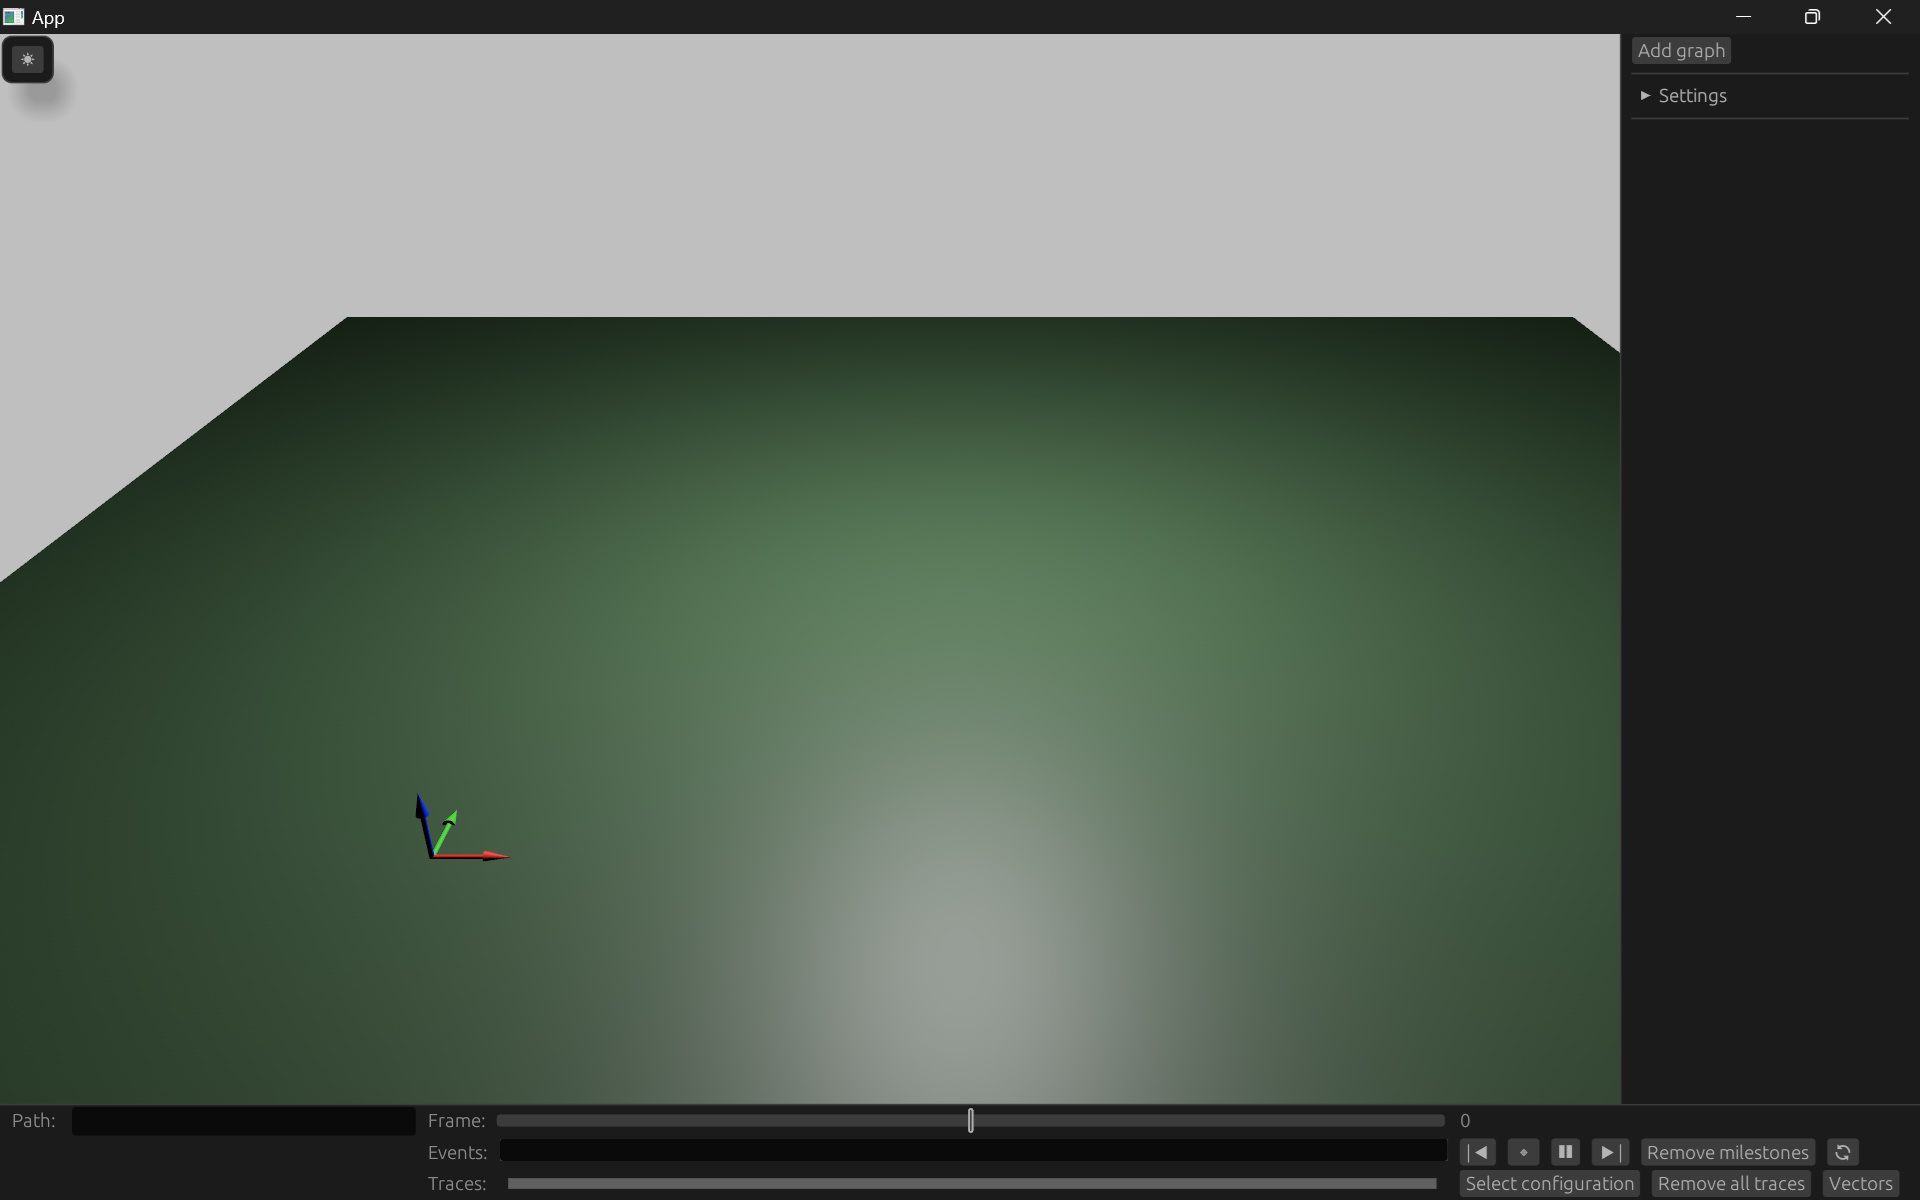
\includegraphics[width=\textwidth]{imagenes/modo_claro.png}
  \caption{Entorno en modo claro}
  \label{fig:modo_claro}
\end{figure}

\subsection{Configuración del entorno} \label{sec:bevy-configuracion}

El proyecto está configurado de manera que al arrancar el programa, se genera un entorno tridimensional vacío, con un plano central, una cámara y una luz. El plano central es un plano de referencia que permite al usuario orientarse en el espacio tridimensional. Tiene un tamaño de 10x10 metros, y está representado en un color verde oscuro. El foco de luz se sitúa a tres metros por encima del plano, y tiene un color frío. La cámara se sitúa a 7 metros, enfocando al centro del plano. La cámara tiene un color de fondo oscuro, y cambiar entre modo claro y oscuro varía este color.

La implementación de la cámara no se basa en ningún \textit{crate} externo, sino que se ha implementado de manera manual para adaptarse al proyecto. Una cámara típicamente tiene tres variables que controlar, que son el \textit{yaw}, el \textit{pitch} y el \textit{roll}. El \textit{yaw} es la rotación de la cámara alrededor del eje vertical (Y), el \textit{pitch} es la rotación de la cámara alrededor del eje lateral (X), y el \textit{roll} es la rotación de la cámara alrededor del eje longitudinal (Z). En este caso, es necesario que el \textit{roll} sea cero, puesto que el entorno es un plano. Tanto el \textit{yaw} como el \textit{pitch} se pueden controlar pulsando el botón derecho del ratón y moviendo el ratón. Además, se puede controlar la posición de la cámara pulsando el botón izquierdo del ratón y moviendo el ratón. Esto permite al usuario moverse por el entorno tridimensional de manera intuitiva.


\subsection{Información global} \label{sec:bevy-global}

El programa almacena una serie de información a partir del \ac{C3D} cargado. Esta información se almacena en un \texttt{Resource}, que es una estructura de datos interna, generada automáticamente al arrancar el programa, y que permite gestionar y acceder a la información de manera eficiente. Esta estructura tiene el nombre de \texttt{AppState}, y contiene la información global necesaria para el funcionamiento del programa, incluyendo el \textit{frame} actual, el número de \textit{frames} del \ac{C3D}, el \textit{path} al fichero \ac{C3D}, el \textit{path} al fichero de configuración, la tasa de refresco del \ac{C3D}, la tasa de refresco seleccionada por el usuario, y diferentes booleanos que contienen información sobre el estado del programa, como si se está reproduciendo o no.


\subsection{Orientación a eventos} \label{sec:bevy-eventos}

Este proyecto tiene un enfoque orientado a eventos. Esto significa que el programa reacciona a los eventos que ocurren en el entorno, como la carga de un fichero o la interacción del usuario. 

Un evento en \textit{Bevy} es una estructura de datos que representa una acción o un cambio en el estado del programa. Estos eventos pueden ser generados por el usuario, como pulsar un botón o mover el ratón, o por el propio programa, como la carga de un fichero o la actualización de la escena. Cuando ocurre un evento, \textit{Bevy} reacciona en la siguiente iteración de su bucle interno, lo que implica que tiene efecto en la siguiente actualización de la imagen, que típicamente coincidirá con el siguiente \textit{frame}.

Los eventos definidos en este proyecto se agrupan en seis enumerados, que se reúnen en la \autoref{tab:enum-eventos}:

\begin{table}[H]
  \centering
  % \setlength{\tabcolsep}{5pt}
  \rowcolors{2}{white}{gray!10}
  \begin{tabular}{c|c}
  \toprule
  {\textbf{Grupo}} & {\textbf{Relación}} \\
  \midrule
  MarkerEvent & Marcadores \\
  JoinsEvent & Uniones \\
  VectorEvent & Vectores \\
  TraceEvent & Trazas \\
  MilestoneEvent & Eventos \\
  GraphEvent & Interfaz gráfica \\
  \bottomrule
  \end{tabular}
  \caption{Grupos de eventos definidos en el programa}
  \label{tab:enum-eventos}
\end{table}

Cada grupo de eventos cuenta con un orquestador encargado de tomar las acciones pertinentes dependiendo del subtipo de evento. Rust facilita el manejo de eventos de este tipo, puesto que cada grupo se codifica como un \texttt{enum}, que define diferentes variantes.

En resumen, los eventos definidos en el programa se agrupan en la \autoref{tab:eventos}. Esta tabla resume las acciones que puede realizar un usuario al interaccionar con la aplicación.

\begin{table}[H]
  \centering
  % \setlength{\tabcolsep}{5pt}
  \rowcolors{2}{white}{gray!10}
  \begin{tabular}{c|c}
  \toprule
  {\textbf{Evento}} & {\textbf{Significado}} \\
  \midrule
  DespawnAllMarkersEvent & Elimina todos los marcadores \\
  DespawnAllJoinsEvent & Elimina todas uniones representadas \\
  DespawnJoinEvent(String, String) & Elimina la unión entre dos marcadores \\
  HideAllVectorsEvent & Esconder todos los vectores \\
  ShowAllVectorsEvent & Mostrar todos los vectores \\
  HideVectorEvent(Vector) & Esconder un vector \\
  ShowVectorEvent(Vector) & Mostrar un vector \\  
  AddTraceEvent(String) & Añade la traza de un marcador \\
  UpdateTraceEvent & Recargar las traza \\
  DespawnTraceEvent(String) & Eliminar la traza de un marcador \\
  DespawnAllTracesEvent & Eliminar todas las trazas\\
  AddMilestoneFromC3dEvent(usize) & Añade un evento en un \textit{frame} \\
  RemoveMilestoneEvent(usize) & Elimina el evento de un \textit{frame} \\
  RemoveAllMilestonesEvent & Elimina todos los eventos \\
  AddGraph(String, XYZ) & Crea un gráfico \\
  RemoveGraph(String) & Elimina un gráfico \\
  RestartGraphs & Reinicia los gráficos \\
  CreateMarkersWindow & Crea la ventana de selección \\  
  \bottomrule
  \end{tabular}
  \caption{Eventos definidos en el programa}
  \label{tab:eventos}
\end{table}

\section{Fichero de configuración \acs{TOML}}

El fichero de configuración de este proyecto define el modo de representación del fichero \ac{C3D} en el entorno 3D. 

Al igual que en el fichero de configuración de Vicon, explicado en \autoref{sec:ficheros-configuracion}, se definen las posibles configuraciones entre corchetes. Cualquier configuración cuenta con un grupo de puntos visibles (\textit{visible\_points}), un grupo de uniones (\textit{joins}) y un grupo de vectores (\textit{vectors}).

Estos grupos son opcionales, y pueden aparecer en cualquier orden. En caso de no aparecer, el programa no los representará.

\subsection{Configuración básica}

Una posible configuración se muestra en el \autoref{lst:ajuste-simple}.

\begin{lstlisting}[style=mystyle, caption={Ejemplo simple de un fichero de configuración}, label={lst:ajuste-simple}]
[config1]
  visible_points = [
    "LFHD", "RFHD", "RBHD", "LBHD"
  ]
  joins = [
    ["LFHD", "RFHD", "RBHD", "LBHD", "LFHD"]
  ]
\end{lstlisting}

En el fragmento anterior, se muestra una configuración sencilla, \texttt{config1}, que representa los marcadores \ac{LFHD}, \ac{RFHD}, \ac{RBHD} y \ac{LBHD} como puntos visibles. Después, se define una unión entre los cuatro marcadores. Para representar un cuadrado, se duplica el primer marcador, \ac{LFHD}, al final de la lista. De este modo, se cierra la unión entre los cuatro marcadores. Además, se puede apreciar que en el grupo de uniones aparece un corchete extra. Esto se debe a que el grupo se considera una lista de listas. Las listas hijas representan diferentes uniones, es decir, grupos independientes de marcadores que se unen entre sí.

Estos cuatro marcadores representan los puntos de la cabeza. Es una combinación muy común, que posiblemente se utilice en varias configuraciones. Para facilitar su uso, el fichero de configuración permite definir un grupo de marcadores como un alias. De este modo, se puede definir el grupo de marcadores de la cabeza como \texttt{head}, y usarlo de la manera definida en el \autoref{lst:grupos-puntos}, donde se muestra un ejemplo de cómo definir grupos de puntos, mediante la palabra reservada \textit{point\_groups}. En este caso, se definen dos grupos, \texttt{head} y \texttt{shoulders}. La forma de indicar al programa que se está referenciando a un grupo de puntos en vez de a un marcador es envolviendo al nombre entre corchetes.

En la configuración \texttt{config1}, se representa el grupo de la cabeza como un punto visible y como una unión. Nótese que al usar el grupo de puntos de la cabeza, se está incluyendo dos veces el punto \ac{LFHD}. Esto no es relevante, dado que internamente el programa trata este punto como uno solo, al usarse como clave de un \textit{Hashmap}, que no permite la duplicación de elementos. En la configuración \texttt{config2}, se representan ambos grupos como puntos visibles y como uniones independientes. 

\newpage

\begin{lstlisting}[style=mystyle, caption={Ejemplo de un grupo de puntos}, label={lst:grupos-puntos}]
[point_groups]
  head = ["LFHD", "RFHD", "RBHD", "LBHD", "LFHD"]
  shoulders = ["LSHO", "RSHO"]

[config1]
  visible_points = [
    ["head"]
  ]
  joins = [
    [["head"]]
  ]
[config2]
  visible_points = [
    ["head"], ["shoulders"]
  ]
  joins = [
    [["head"]], 
    [["shoulders"]]
  ]
\end{lstlisting}

\subsection{Personalización general: Color y tamaño}

El fichero de configuración permite personalizar la representación de los marcadores. Para ello, se definen una serie de palabras reservadas. Estas palabras son \texttt{point\_color}, \texttt{point\_size}, \texttt{join\_color} y \texttt{line\_thickness}. Estas palabras son opcionales, y permiten personalizar la representación de los marcadores y las uniones. Los colores se pueden definir en formato rgb, como una lista de tres números enteros entre 0 y 255, o como rgb con transparencia, como una lista de cuatro números enteros entre 0 y 255.

En el \autoref{lst:cfg-personalizada} se muestra un ejemplo de la personalización de una configuración, sobreescribiendo los valores por defecto. En este caso, para la configuración \texttt{config1}, los marcadores se representan en rojo, y las uniones en verde. Cada línea se representa con el doble de grosor que el valor por defecto, y los marcadores tienen un tamaño 1.5 veces mayor que el valor por defecto. En la configuración \texttt{config2}, los marcadores se representan en azul, con un 40\% de transparencia, y el doble de tamaño que el valor por defecto. Las uniones no se personalizan, por lo que se usan los valores por defecto.

\begin{lstlisting}[style=mystyle, caption={Configuración personalizada}, label={lst:cfg-personalizada}]
[point_groups]
  head = ["LFHD", "RFHD", "RBHD", "LBHD", "LFHD"]
  shoulders = ["LSHO", "RSHO"]

[config1]
  visible_points = [
    ["head"]
  ]
  joins = [
    [["head"]]
  ]
  point_color = [255, 0, 0]
  join_color = [0, 0, 255]
  line_thickness = 2.0
  point_size = 1.5

[config2]
  visible_points = [
    ["head"], ["shoulders"]
  ]
  joins = [
    [["head"]], 
    [["shoulders"]]
  ]
  point_color = [0, 0, 255, 100]
  point_size = 2.0
\end{lstlisting}

Lo visto en el \autoref{lst:cfg-personalizada} es un ejemplo de sobreescritura de los valores por defecto para cada configuración. Sin embargo, se puede lograr una personalización más extrema gracias a los grupos de puntos, a los que se les pueden aplicar las mismas palabras reservadas. De este modo, se pueden definir diferentes colores y tamaños para cada grupo de puntos. En el \autoref{lst:cfg-grupos-personalizados} se muestra un ejemplo de cómo personalizar los grupos de puntos:

\begin{lstlisting}[style=mystyle, caption={Configuración personalizada de grupos de puntos}, label={lst:cfg-grupos-personalizados}]
[point_groups]
  head = ["LFHD", "RFHD", "RBHD", "LBHD", "LFHD"]
  shoulders = ["LSHO", "RSHO"]

[head.config]
  point_color = [255, 0, 0]
  point_size = 0.5
  join_color = [255, 128, 0]

[config1]
  visible_points = [
    ["head"]
  ]
  joins = [
    [["head"]]
  ]
  point_color = [255, 0, 0]
  join_color = [0, 0, 255]
  line_thickness = 2.0
  point_size = 1.5

[config2]
  visible_points = [
    ["head"], ["shoulders"]
  ]
  joins = [
    [["head"]], 
    [["shoulders"]]
  ]
  point_color = [0, 0, 255, 100]
  point_size = 2.0
\end{lstlisting}

Como se puede apreciar, se utiliza el nombre del grupo de puntos seguido de \texttt{.config} para definir la configuración de ese grupo, sobreescribiendo el valor por defecto de su configuración. En este caso, el grupo de puntos \texttt{head} se representa en rojo, con un tamaño de 0.5 veces el valor por defecto, y las uniones en naranja. El grupo de puntos \texttt{shoulders} no se personaliza, por lo que se usan los valores por defecto, que será azul en \texttt{config1} y verde en \texttt{config2}, puesto que verde es el color por defecto para las uniones, y en \texttt{config2} no se está sobreescribiendo.

\subsection{Personalización avanzada: Formas}

Las uniones entre dos marcadores se generan por defecto mediante un cilindro delgado, con apariencia de una línea. Mediante la palabra reservada \texttt{line\_thickness} se puede modificar este comportamiento, pero adicionalmente se puede modificar la forma. Las otras figuras admitidas son: un cono, un semicono y un prisma rectangular.

\begin{lstlisting}[style=mystyle, caption={Uso de formas}, label={lst:cfg-formas}] 
[config1]
  joins = [
    { points = ["RSJC", "RELJ"], shape = { type = "cone", radius = 1 } },
    { points = ["RELJ", "RWJC"], shape = { type = "semicone", radius1 = 4.0, radius2 = 2.0 } },
    { points = ["LSJC", "LELJ", "LWJC"], shape = { type = "prism", width = 4.0, height = 2.0 } },
  ]
\end{lstlisting}

Cada forma dispone de sus propias palabras reservadas, y las mayúsculas son irrelevantes (\textit{Case insensitive}). 

En el caso del cono, solo se debe especificar el radio, que define el tamaño de la circunferencia del primer elemento de la unión (en este caso \texttt{RSJC}). Además, cada forma tiene sinónimos, esto es, palabras que significan lo mismo para el programa. En el caso de ``cone'', se puede especificar también en español (``cono'').

En el caso del semicono, se deben especificar dos radios, que definen el tamaño de las dos circunferencias. Además, sinónimos de ``semicone'' son: ``semicono'', ``cone frustum'', ``cono truncado'', ``partial cone'', ``cono parcial'', ``truncated cone'' y ``cono truncado''.

En el caso del prisma rectangular, se deben especificar dos dimensiones, que definen el tamaño de las dos bases del prisma. Además, sinónimos de ``prism'' son: ``prisma'', ``rectangular prism'', ``prisma rectangular'', ``paralelepipedo'', ``paralelepípedo'' y ``parallelepiped''.

\subsection{Configuración de vectores}

Los vectores son similares a los vectores de referencia explicados en \autoref{sec:bevy}. En el fichero de configuración, se definen como un punto de anclaje, una lista de elementos anclados a ese marcador, y opcionalmente una escala. Los vectores permiten representar relaciones espaciales y se pueden utilizar para definir trayectorias o movimientos en el espacio tridimensional.

\begin{lstlisting}[style=mystyle, caption={Configuración de un vector}, label={lst:cfg-vector}]
[config1]
  vectors = [ 
    ["OBJ1", "LVelOBJ1"],
    ["LUarmCM", ["LUarmIv", "LUarmJv", "LUarmKv"], 2.5],
    ["RUarmCM", ["RUarmIv", "RUarmJv"], 2.5],
    ["RUarmCM", "RUarmKv", 1.5],
]
\end{lstlisting}

En el \autoref{lst:cfg-vector} se muestra un ejemplo de como configurar vectores. En este caso, se han definido tres puntos de anclaje: \texttt{OBJ1}, \texttt{LUarmCM} y \texttt{RUarmCM}. 

El primero de ellos, \texttt{OBJ1}, tiene un solo elemento anclado, \texttt{LVelOBJ1}. Esta configuración ancla el marcador de representación de la velocidad de LVelOBJ1 a OBJ1. Esto representará un vector tangente a la trayectoria del objeto en cualquier punto.

El segundo, \texttt{LUarmCM}, tiene tres elementos anclados, \texttt{LUarmIv}, \texttt{LUarmJv} y \texttt{LUarmKv}, y una escala de 2.5. Esta es una configuración estándar para la representación de un sistema de coordenadas local, que sirven para cuantificar la rotación de un marcador.

El tercero, \texttt{RUarmCM}, tiene tres elementos anclados, \texttt{RUarmIv} y \texttt{RUarmJv}, con una escala de 2.5, y posteriormente se añade el tercer elemento, \texttt{RUarmKv}, con una escala de 1.5. Similar al caso anterior, se representa un sistema de coordenadas local, pero reduciendo el tamaño de la componente K.

Los vectores tienen una configuración de color fija. Para los vectores que tienen un número diferente a tres elementos anclados, se representan en amarillo, mientras que si el número de marcadores anclados a un punto es exactamente igual a tres, el programa entiende que se trata de una representación de vectores de referencia, para lo que utiliza colores estándar en otros motores de videojuegos, representando la primera componente en rojo, la segunda en verde y la tercera en azul. 

\subsection{Expresiones regulares}

A la hora de leer el fichero de configuración, se utilizan expresiones regulares para determinar si un marcador debe representarse o no. Esto permite representar un grupo de marcadores sin necesidad de definirlos uno a uno. Sin embargo, esto podría causar que se añadan más marcadores de los deseados. Por ejemplo, si se incluye el marcador \texttt{OBJ1}, se podría incluir también \texttt{LVelOBJ1}. 

Para evitar esto, el programa rodea el nombre del marcador con el símbolo \texttt{\^} al principio y el símbolo \texttt{\$} al final. De este modo, se asegura que el nombre del marcador coincide exactamente con el nombre del marcador en el fichero \ac{C3D}. Pero podría darse el caso de que se quiera representar ambos marcadores. Para ello, el programa admite un guión bajo (\texttt{\_}) como comodín. De este modo, si se incluye el marcador \texttt{\_OBJ1}, se incluirán todos los marcadores que cumplan la expresión regular, como \texttt{OBJ1} o \texttt{LVelOBJ1}. 

\section{Carga de ficheros}

El fichero de configuración y el fichero \ac{C3D} se cargan de forma simple, arrastrándolo a la ventana del programa. El programa detecta el tipo de fichero y lo carga automáticamente. Se puede variar el fichero \ac{C3D} o el fichero de configuración en tiempo de ejecución, y el programa lo detecta automáticamente.

\textit{Bevy} tiene una función nativa para la captura de los ficheros que se sueltan sobre la ventana. Sin embargo, en la versión web el navegador captura el fichero antes que \textit{Bevy}, por lo que es imposible la carga de ficheros de este modo. Para ello se ha modificado el crate \texttt{bevy\_web\_file\_drop} para darle compatibilidad con la versión 0.15 de \textit{Bevy}, dado que este \textit{crate} está escrito para la versión 0.14 y no presenta compatibilidad \autocite{Bevy_web_file_dropCratesioRust2024}.

Con estas modificaciones, el programa es capaz de capturar un archivo tanto en la versión de escritorio como en la versión web. Para esta última utiliza una \textit{Blob URL} para la carga del fichero \autocite{AnswerWhatBlob2015,FileAPI}.

Cuando un fichero se carga, se toman diferentes acciones, dependiendo de su tipo. Si se trata de un \ac{C3D} se eliminan todos los marcadores y se envía un evento de carga al \textit{parser} de \ac{C3D}. Este \textit{parser} se encarga de cargar el fichero y enviar un evento al programa con los datos cargados. Si se trata de un fichero de configuración, simplemente se indica al programa que debe generar nuevamente las uniones y vectores, sin necesidad de eliminar los marcadores. 

\section{Representación tridimensional} \label{sec:representacion-3d}

La \autoref{fig:flujo} muestra un diagrama de actividad de la representación tridimensional del \ac{C3D} en un entorno de escritorio. Se puede observar como el motor paraleliza diferentes cálculos, como la clasificación de los marcadores, la generación de las uniones y generación de los vectores, así como el cálculo de la posición de las uniones y los vectores. En un entorno web no es posible la paralelización de estos cálculos, por limitaciones actuales de los navegadores en el contexto de \textit{WebAssembly}, donde todas las acciones ocurren dentro de un bucle de \textit{JavaScript}. En este caso, \textit{Bevy} decide el orden de ejecución de los cálculos.

\begin{figure}[H]
  \centering
  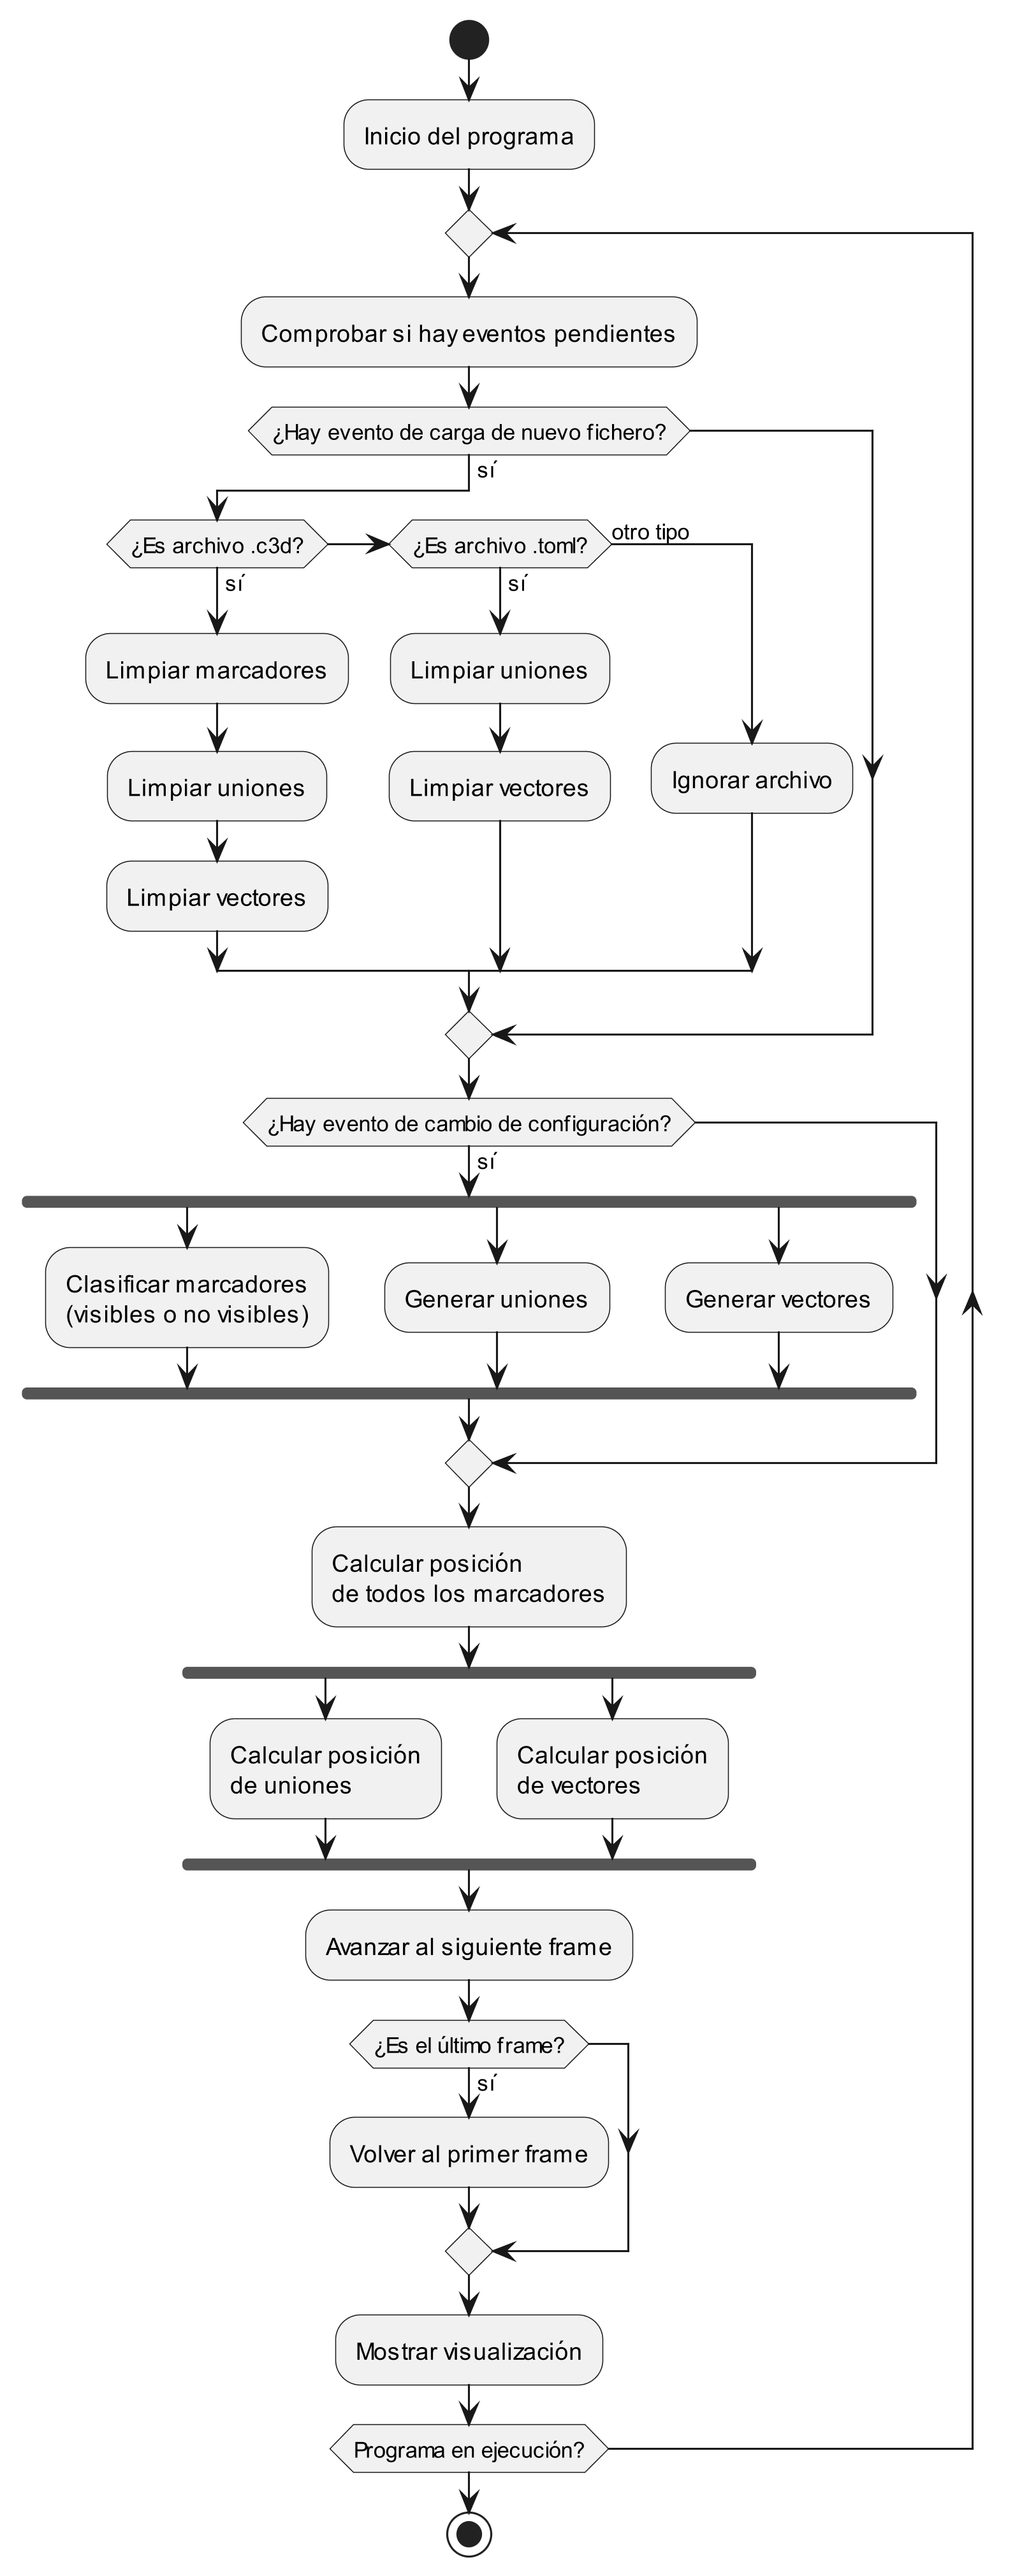
\includegraphics[height=0.9\textheight, keepaspectratio]{imagenes/diagramas/general.png}
  \caption{Diagrama de actividad de la representación del \acs{C3D} en un entorno de escritorio}
  \label{fig:flujo}
\end{figure}

\subsection{Representación de los marcadores} \label{sec:representacion-marcadores}

Los marcadores se representan como esferas, y se pueden personalizar mediante el fichero de configuración. Internamente, el programa utiliza dos estructuras de datos, una contiene el nombre del marcador y su visibilidad, y la otra es una agrupación de marcadores, siguiendo el patrón \ac{ECS} de \textit{Bevy}. Es decir, el componente \texttt{Marker} contiene el nombre del marcador y su visibilidad, mientras que el componente \texttt{C3dMarkers} es únicamente una asignación de una estructura vacía a todos los marcadores. Esto permite eliminar todos los marcadores de forma sencilla, eliminando únicamente el componente padre.

Es necesario mantener en memoria todos los marcadores, incluso los que no son visibles según el fichero de configuración. Esto se debe a que el programa permite cambiar la configuración en tiempo de ejecución, y por tanto, es necesario mantener todos los marcadores en memoria para poder representarlos. Sin embargo, el programa no los representa si no son visibles, gracias a que la estructura de datos contiene la visibilidad de cada marcador\footnote{\textit{Bevy} entiende la visibilidad de cualquier entidad como un enumerado, que puede ser visible, invisible o heredado \autocite{VisibilityBevyRender}.}.

Si se ejecuta el programa sin un fichero de configuración, se representan todos los marcadores como visibles. Esto permite comprobar que el \textit{parser} de \ac{C3D} funciona correctamente, y que se están cargando todos los marcadores. Sin embargo, no se recomienda su uso, dado que el número de marcadores puede ser elevado, y la representación muestra datos que no tienen un sentido espacial. En la \autoref{fig:marcadores} se muestra una imagen de la representación de los marcadores sin un fichero de configuración. Se puede observar que el número de marcadores es elevado, y que aparecen marcadores que no tienen un sentido espacial, como los vectores de velocidad. Por tanto, en la figura se resalta la importancia de la configuración, puesto que es inviable el estudio de un movimiento con un número tan elevado de marcadores. 

\begin{figure}[H]
  \centering
  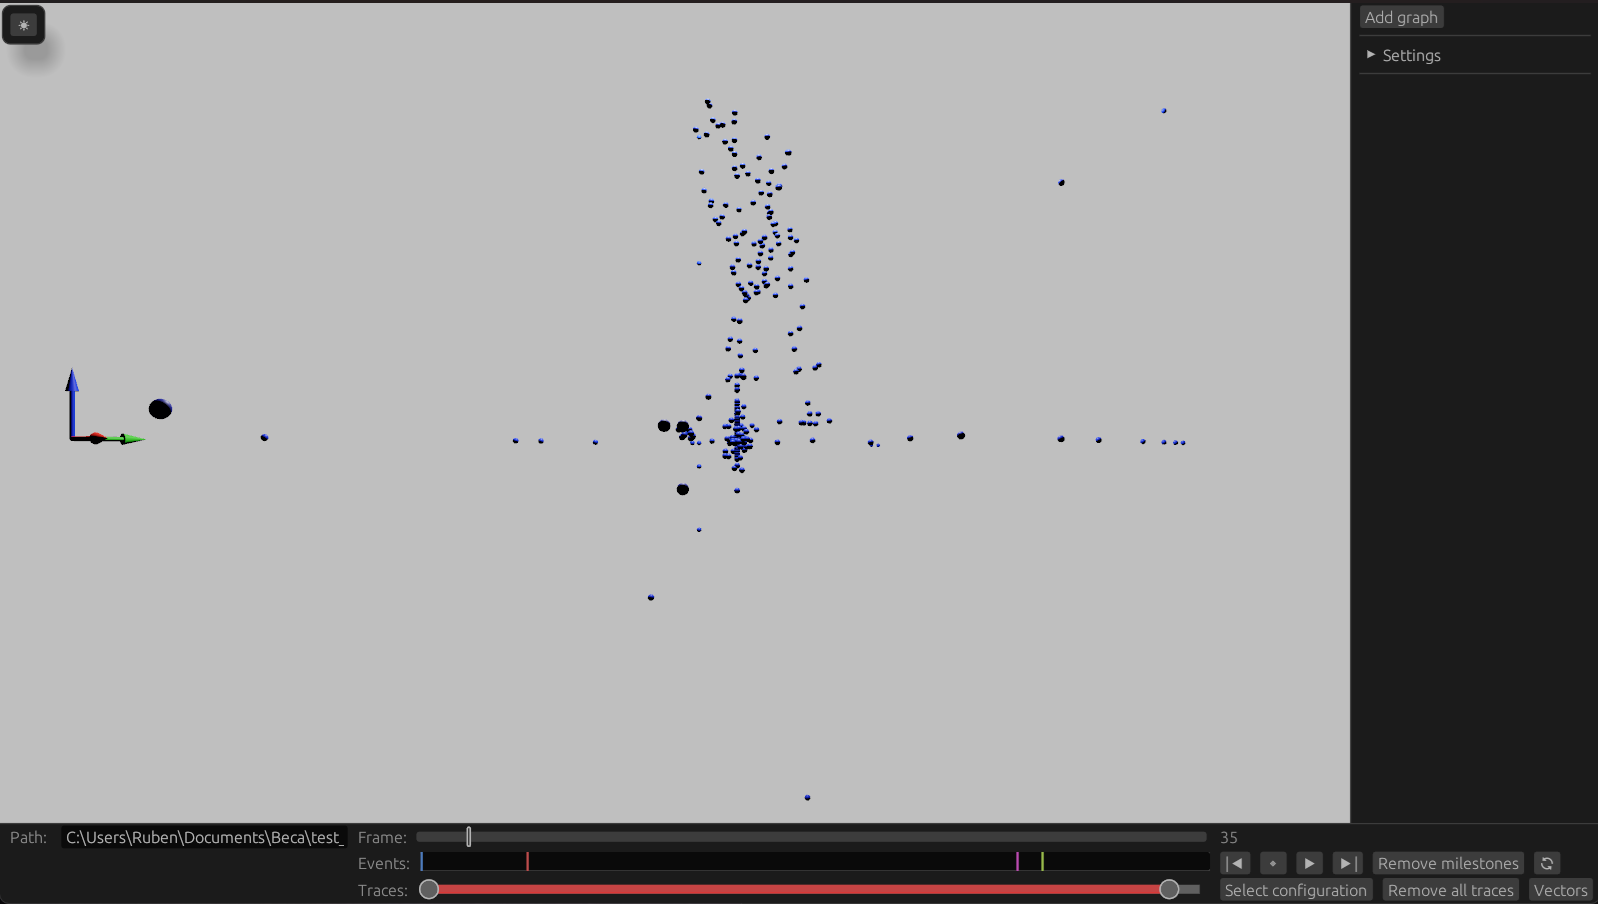
\includegraphics[width=\textwidth]{imagenes/marcadores.png}
  \caption{Representación de marcadores del \acs{C3D} sin un fichero de configuración}
  \label{fig:marcadores}
\end{figure}

Para representar los marcadores, el programa utiliza un componente de \textit{Bevy} llamado \texttt{Mesh}\footnote{Un \textit{mesh} es la estructura tridimensional compuesta por vértices conectados mediante aristas y caras que define la forma geométrica de un objeto 3D, sobre la cual se pueden aplicar materiales y transformaciones para su representación gráfica.}. Este componente permite representar una malla en el espacio tridimensional. En este caso, se utiliza una esfera como malla, con un tamaño y color definidos en el fichero de configuración, o en su defecto, en color azul y con un tamaño por defecto. Si se ha cargado un fichero de configuración, cada marcador se considera visible si aparece en el grupo de puntos visibles. En caso contrario, se considera invisible. De este modo, es sencillo representar solo una parte de los marcadores, y ocultar el resto.

\begin{figure}[H]
  \centering
  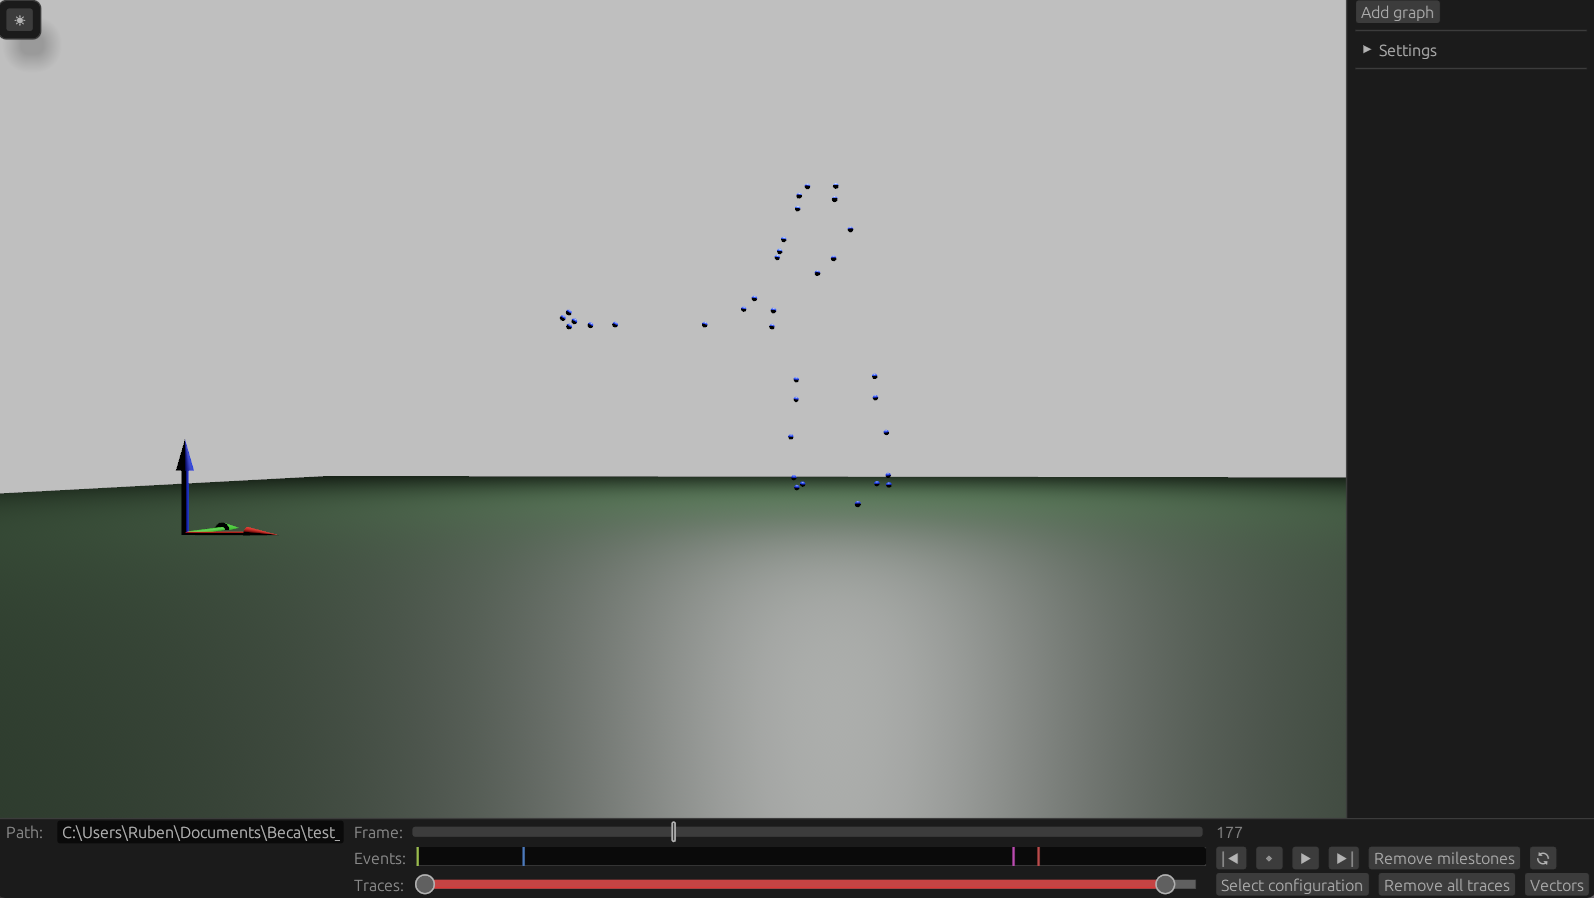
\includegraphics[width=\textwidth]{imagenes/config-basica.png}
  \caption{Representación de marcadores del \acs{C3D} con un fichero de configuración}
  \label{fig:cfg-basica}
\end{figure}

La \autoref{fig:cfg-basica} muestra el mismo fichero que la \autoref{fig:marcadores}, pero filtrando la mayoría de puntos para generar un avatar.

Un diagrama de actividad que explica el funcionamiento de la representación de los marcadores se puede ver en la \autoref{fig:diag-marcadores}.

\begin{figure}[H]
  \centering
  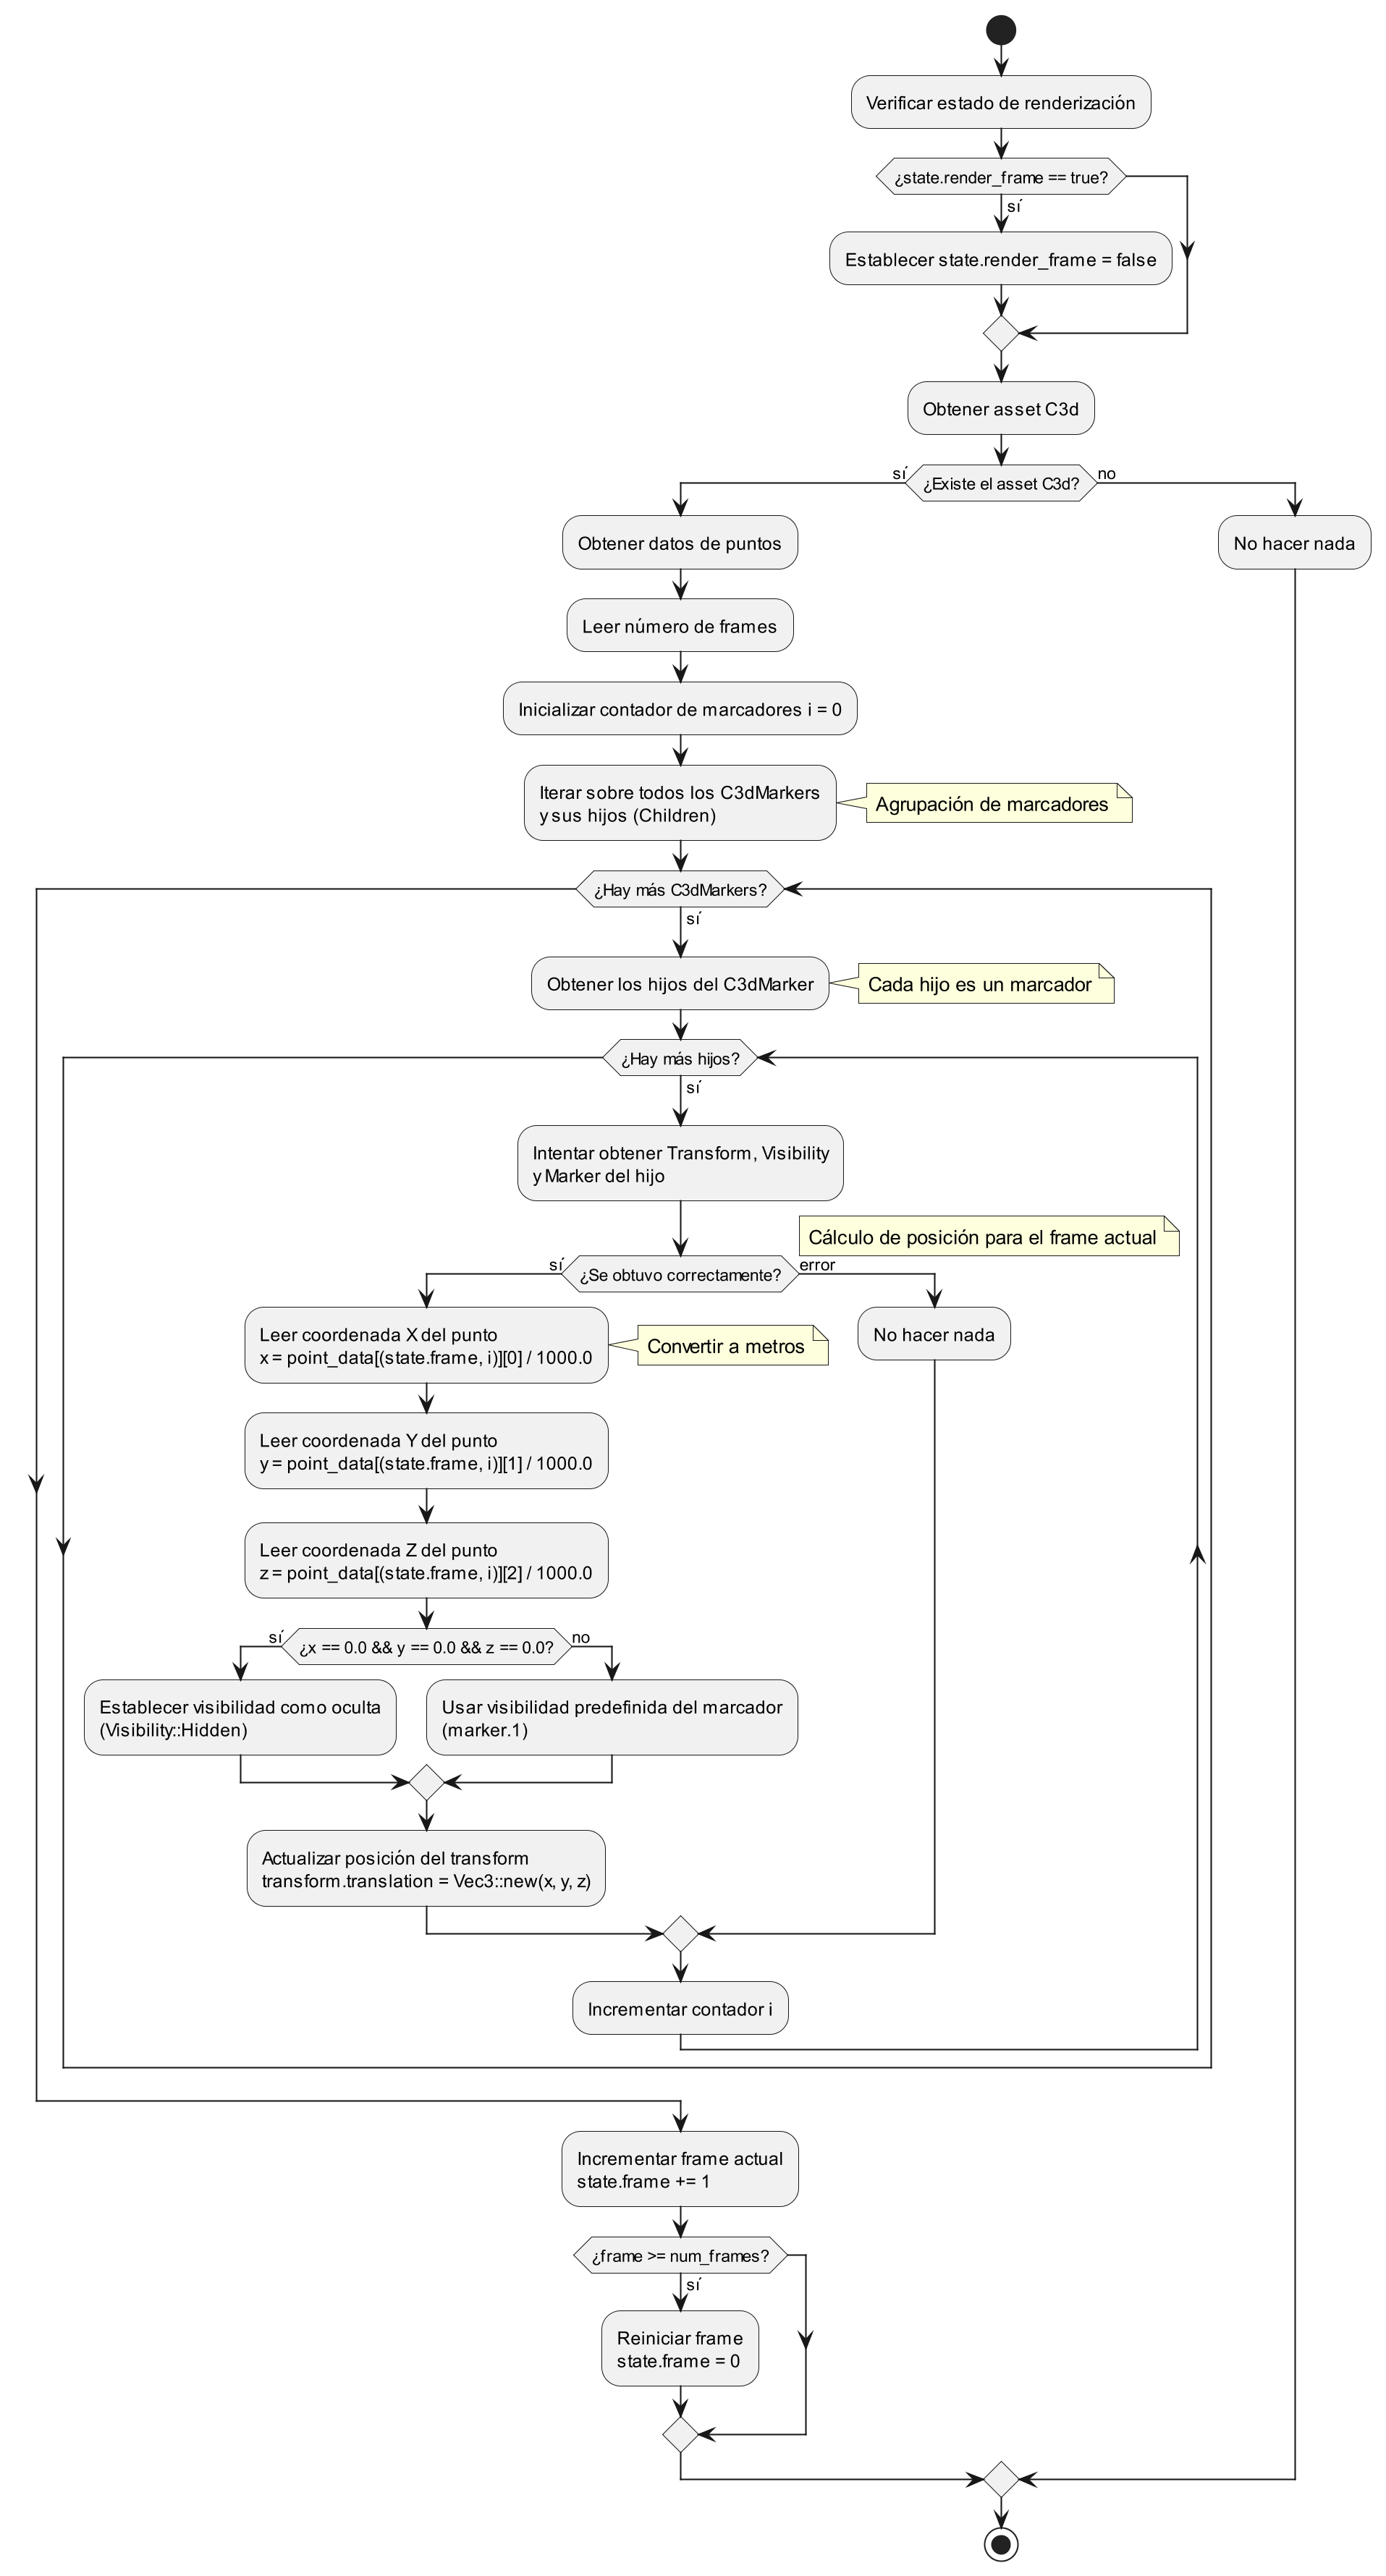
\includegraphics[height=0.9\textheight, keepaspectratio]{imagenes/diagramas/marcadores.png}
  \caption{Diagrama de actividad sobre la representación de los marcadores}
  \label{fig:diag-marcadores}
\end{figure}

\subsection{Representación de las uniones} \label{sec:representacion-uniones}

Las uniones se representan como figuras entre marcadores. Estas figuras pueden ser de diferentes tipos, como un cilindro, un cono, un semicono o un prisma rectangular.

Si se considera la orientación de una unión como un objeto entre dos marcadores, y la rotación de la unión como la magnitud que determina la cara visible, existe un caso particular donde la rotación toma especial relevancia. Este es el caso de que la forma sea un prisma rectangular, ya que con un cilindro o un cono, la rotación no afecta a la representación, pues todas sus caras son iguales. En el caso del prisma rectangular, la rotación se puede determinar mediante los vectores de referencia, que son tres marcadores anclados a un marcador. 

La \autoref{fig:uniones-cilindros} muestra un ejemplo de la representación de las uniones, donde no es importante la rotación de la unión, y la \autoref{fig:uniones-prisma} muestra un ejemplo de la representación de las uniones, donde sí es importante la rotación de la unión dada la forma del prisma rectangular. Además, se muestran los vectores de orientación, que se pueden ocultar, como se explica en \autoref{sec:panel-inferior}

\begin{figure}[H]
  \centering
  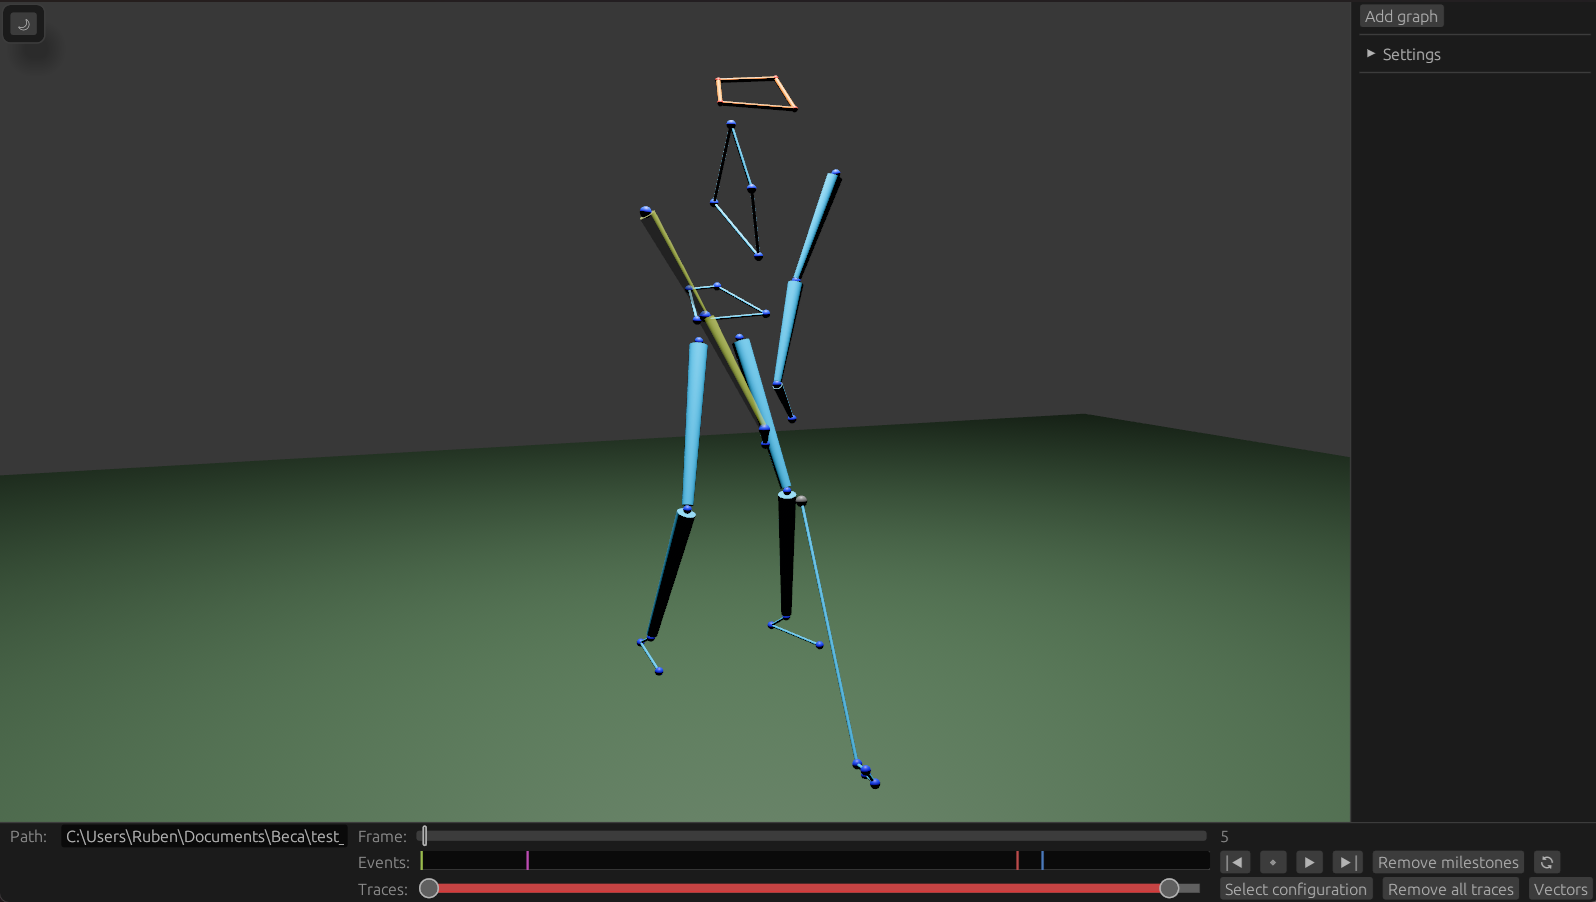
\includegraphics[width=0.8\textwidth]{imagenes/uniones-cilindros.png}
  \caption{Representación de las uniones entre marcadores sin orientación}
  \label{fig:uniones-cilindros}
\end{figure}


\begin{figure}[H]
  \centering
  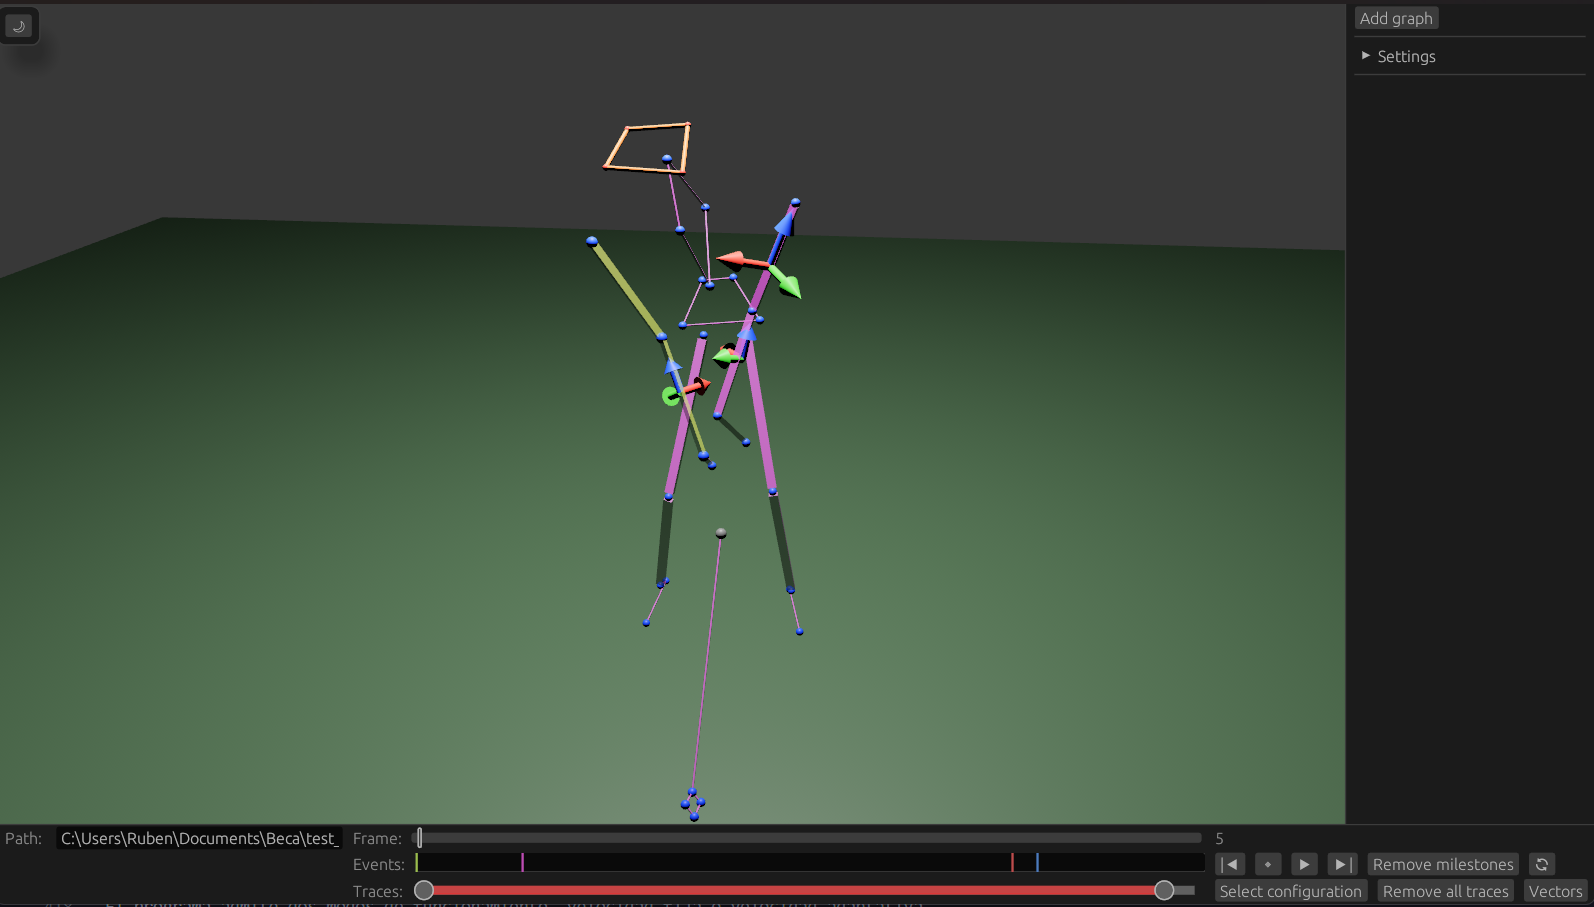
\includegraphics[width=0.8\textwidth]{imagenes/uniones-prisma.png}
  \caption{Representación de las uniones entre marcadores con orientación}
  \label{fig:uniones-prisma}
\end{figure}


Internamente, se trata a las uniones como una estructura de datos que contiene el nombre de los dos marcadores que forman la unión, y la forma de esta. Las uniones se generan cuando se carga una configuración, y se eliminan si se cambia de configuración o se carga un nuevo \ac{C3D}. Esto permite mantener en memoria solo las uniones visibles, y además se reduce el número de cálculos necesarios para representar las uniones en cada fotograma. La \autoref{fig:diag-uniones} muestra un diagrama de actividad que explica el funcionamiento de la representación de las uniones. 

\begin{figure}[H]
  \centering
  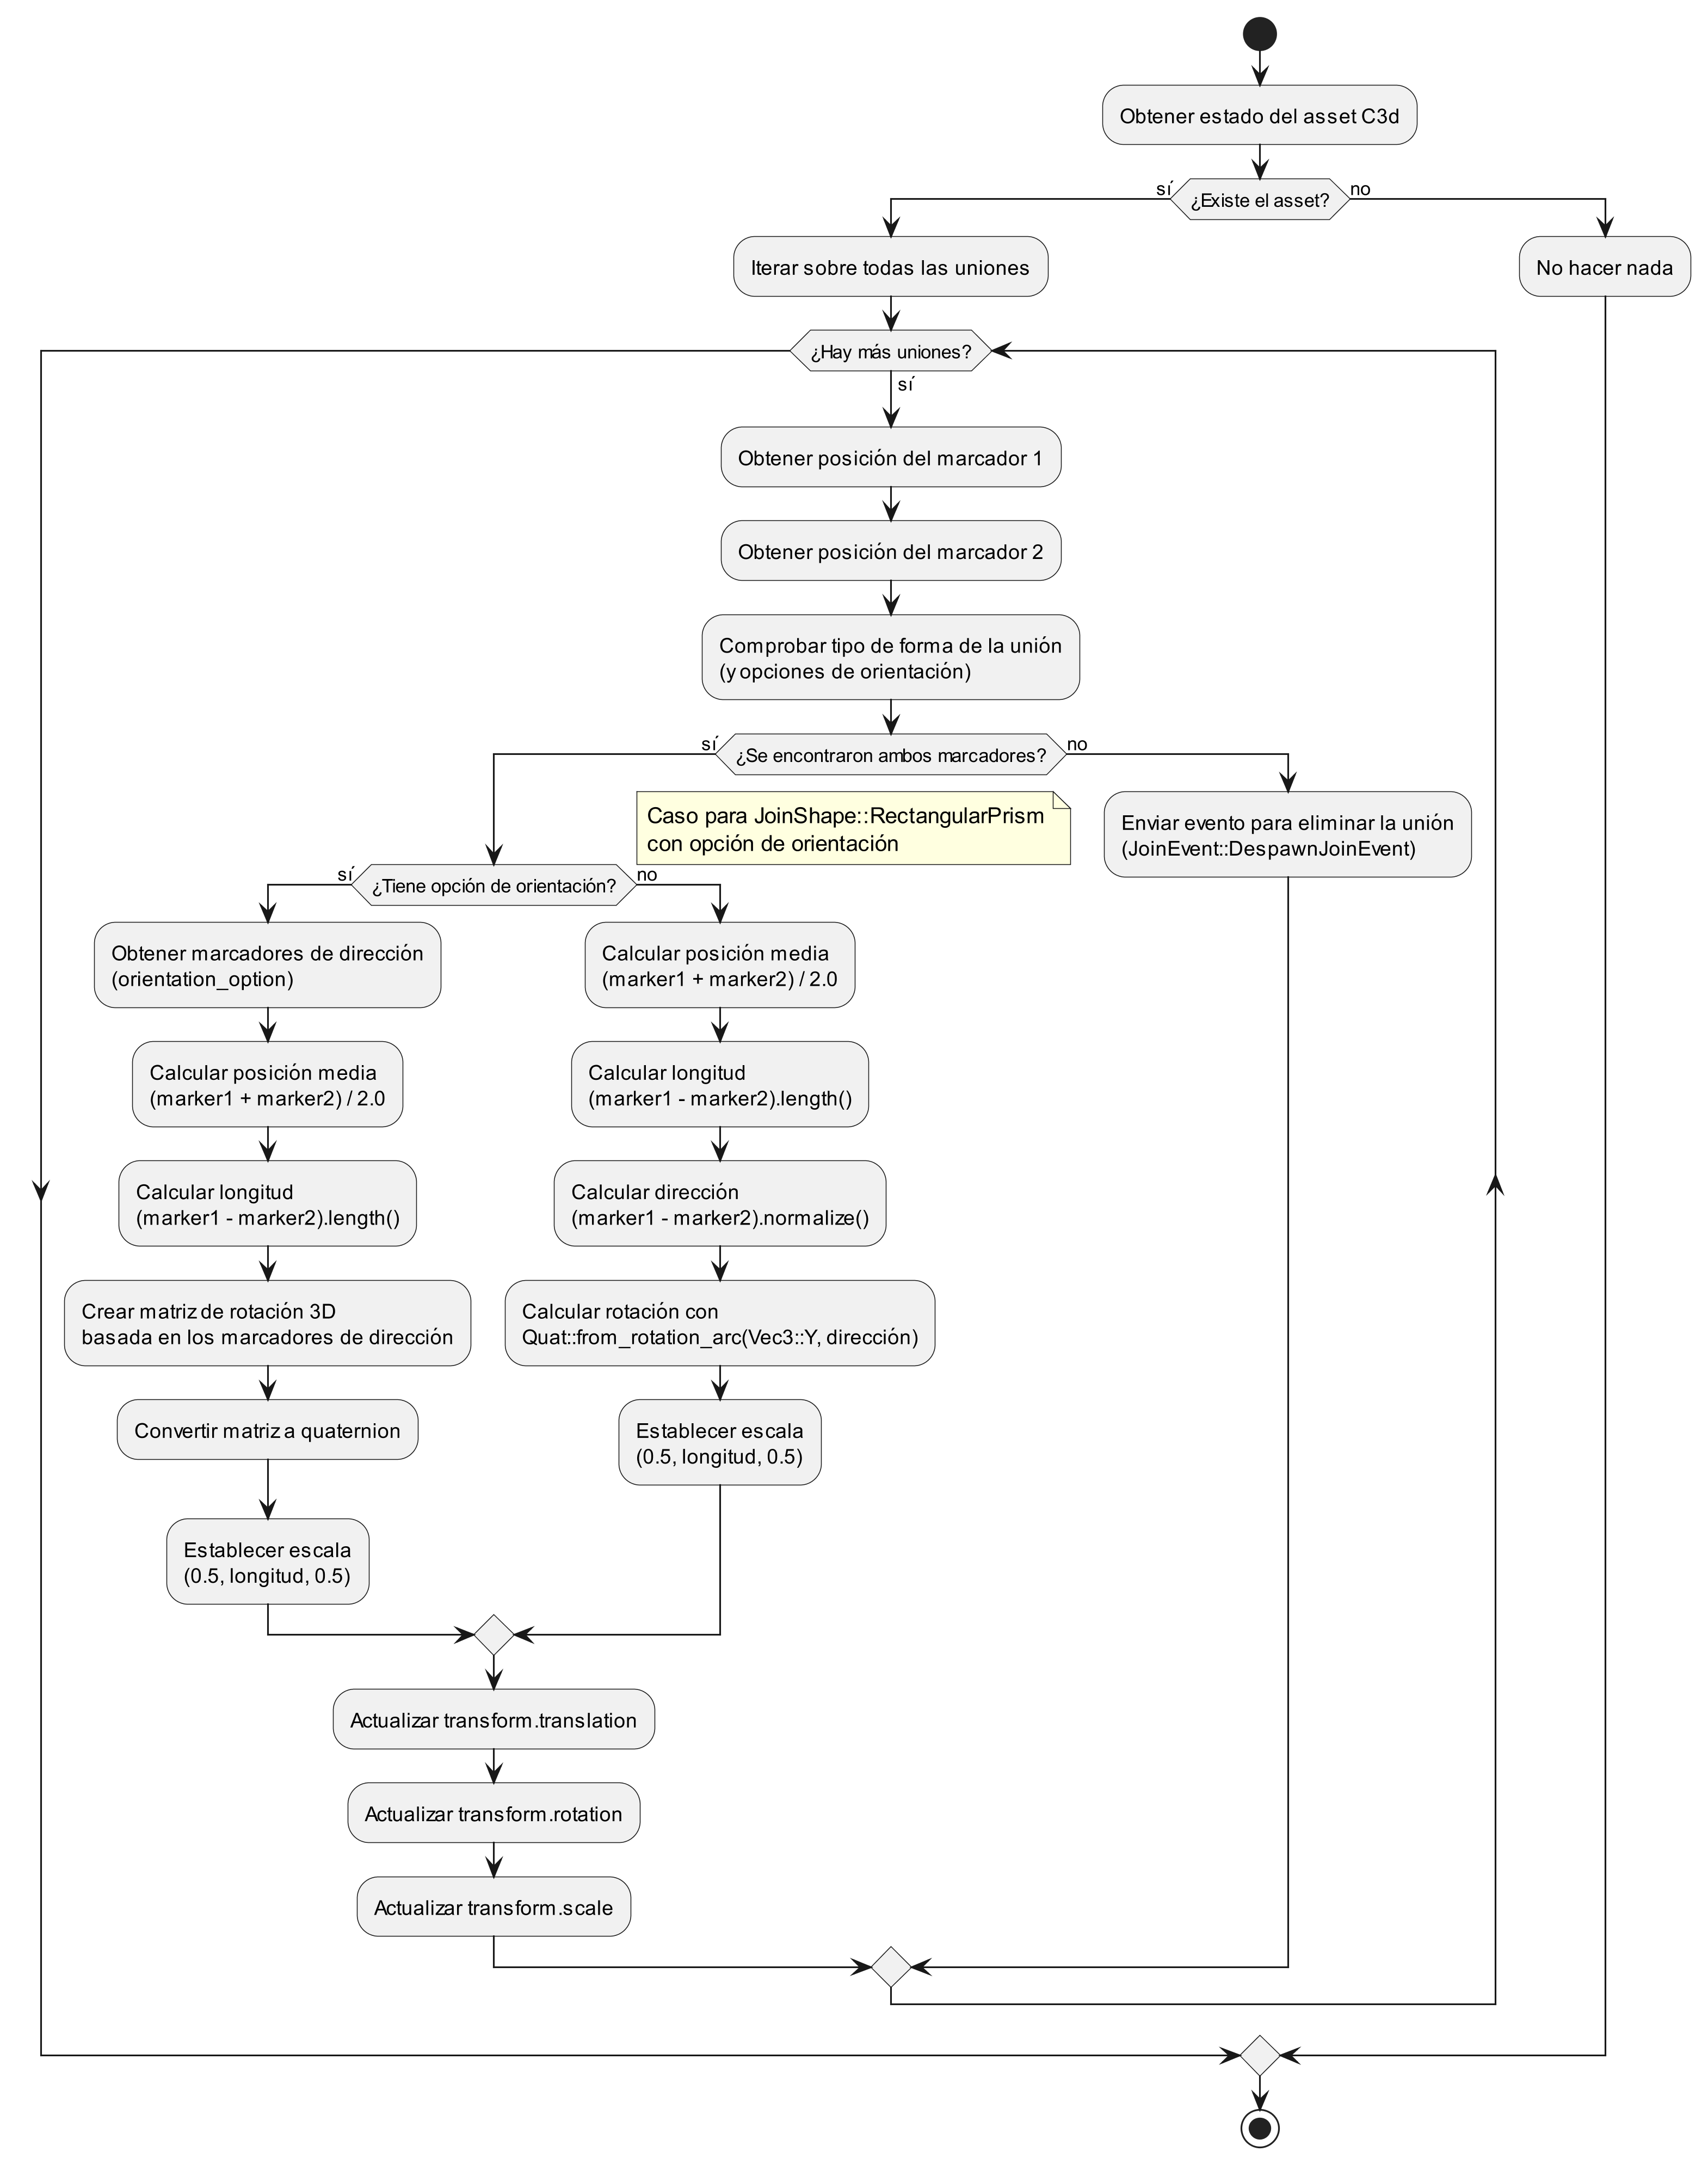
\includegraphics[width=\textwidth]{imagenes/diagramas/uniones.png}
  \caption{Diagrama de actividad sobre la representación de las uniones}
  \label{fig:diag-uniones}
\end{figure}

\subsection{Representación de los vectores} \label{sec:representacion-vectores}

Los vectores se representan como flechas que parten de un marcador, y tienen la dirección, módulo y sentido del vector, representado en el \ac{C3D} como otro marcador. Estos vectores se deben haber calculado previamente, mediante herramientas como \textit{BodyBuilder}\footnote{\textit{BodyBuilder} es una herramienta de Vicon, basada en un lenguaje de scripting, que permite definir modelos cinemáticos y calcular variables biomecánicas a partir de los datos de marcadores capturados en sistemas de análisis de movimiento.}.

Si tomamos como ejemplo un punto de anclaje \texttt{OBJ1}, y su vector de velocidad \texttt{LVelOBJ1}, el programa representa una flecha que parte de \texttt{OBJ1} y tiene la dirección, módulo y sentido del vector \texttt{LVelOBJ1}.

En la \autoref{fig:vectores} se muestra un ejemplo de la representación de los vectores del \ac{C3D}. En este caso, se han representado dos vectores, \texttt{LVelOBJ2}, anclado a \texttt{OBJ2}\footnote{En el fichero \ac{C3D} que se utiliza como ejemplo en esta memoria, los marcadores que comienzan por \texttt{OBJ} representan un punto del palo de golf.} y \texttt{WThorax}, anclado a \texttt{Thorax}. El primero de ellos representa la velocidad de \texttt{OBJ2}, y el segundo representa la velocidad angular del \texttt{Thorax}.

\begin{figure}[H]
  \centering
  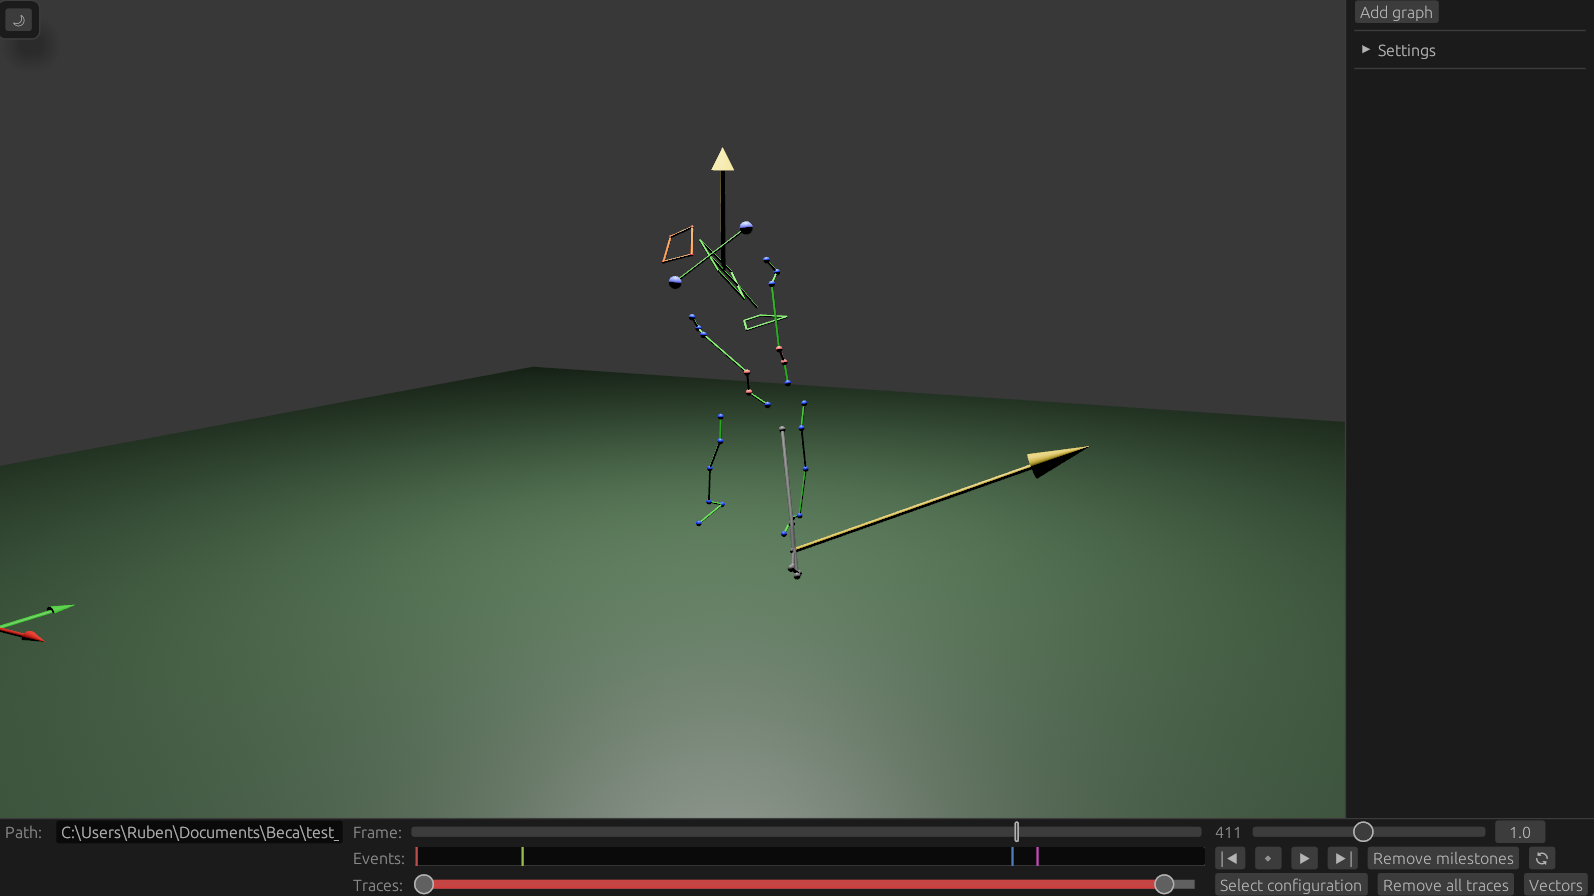
\includegraphics[width=\textwidth]{imagenes/vectores.png}
  \caption{Representación de los vectores del \acs{C3D}}
  \label{fig:vectores}
\end{figure}

La representación de los vectores se ha programado de la forma que se puede ver en el diagrama de actividad de la \autoref{fig:diag-vectores}.

\begin{figure}[H]
  \centering
  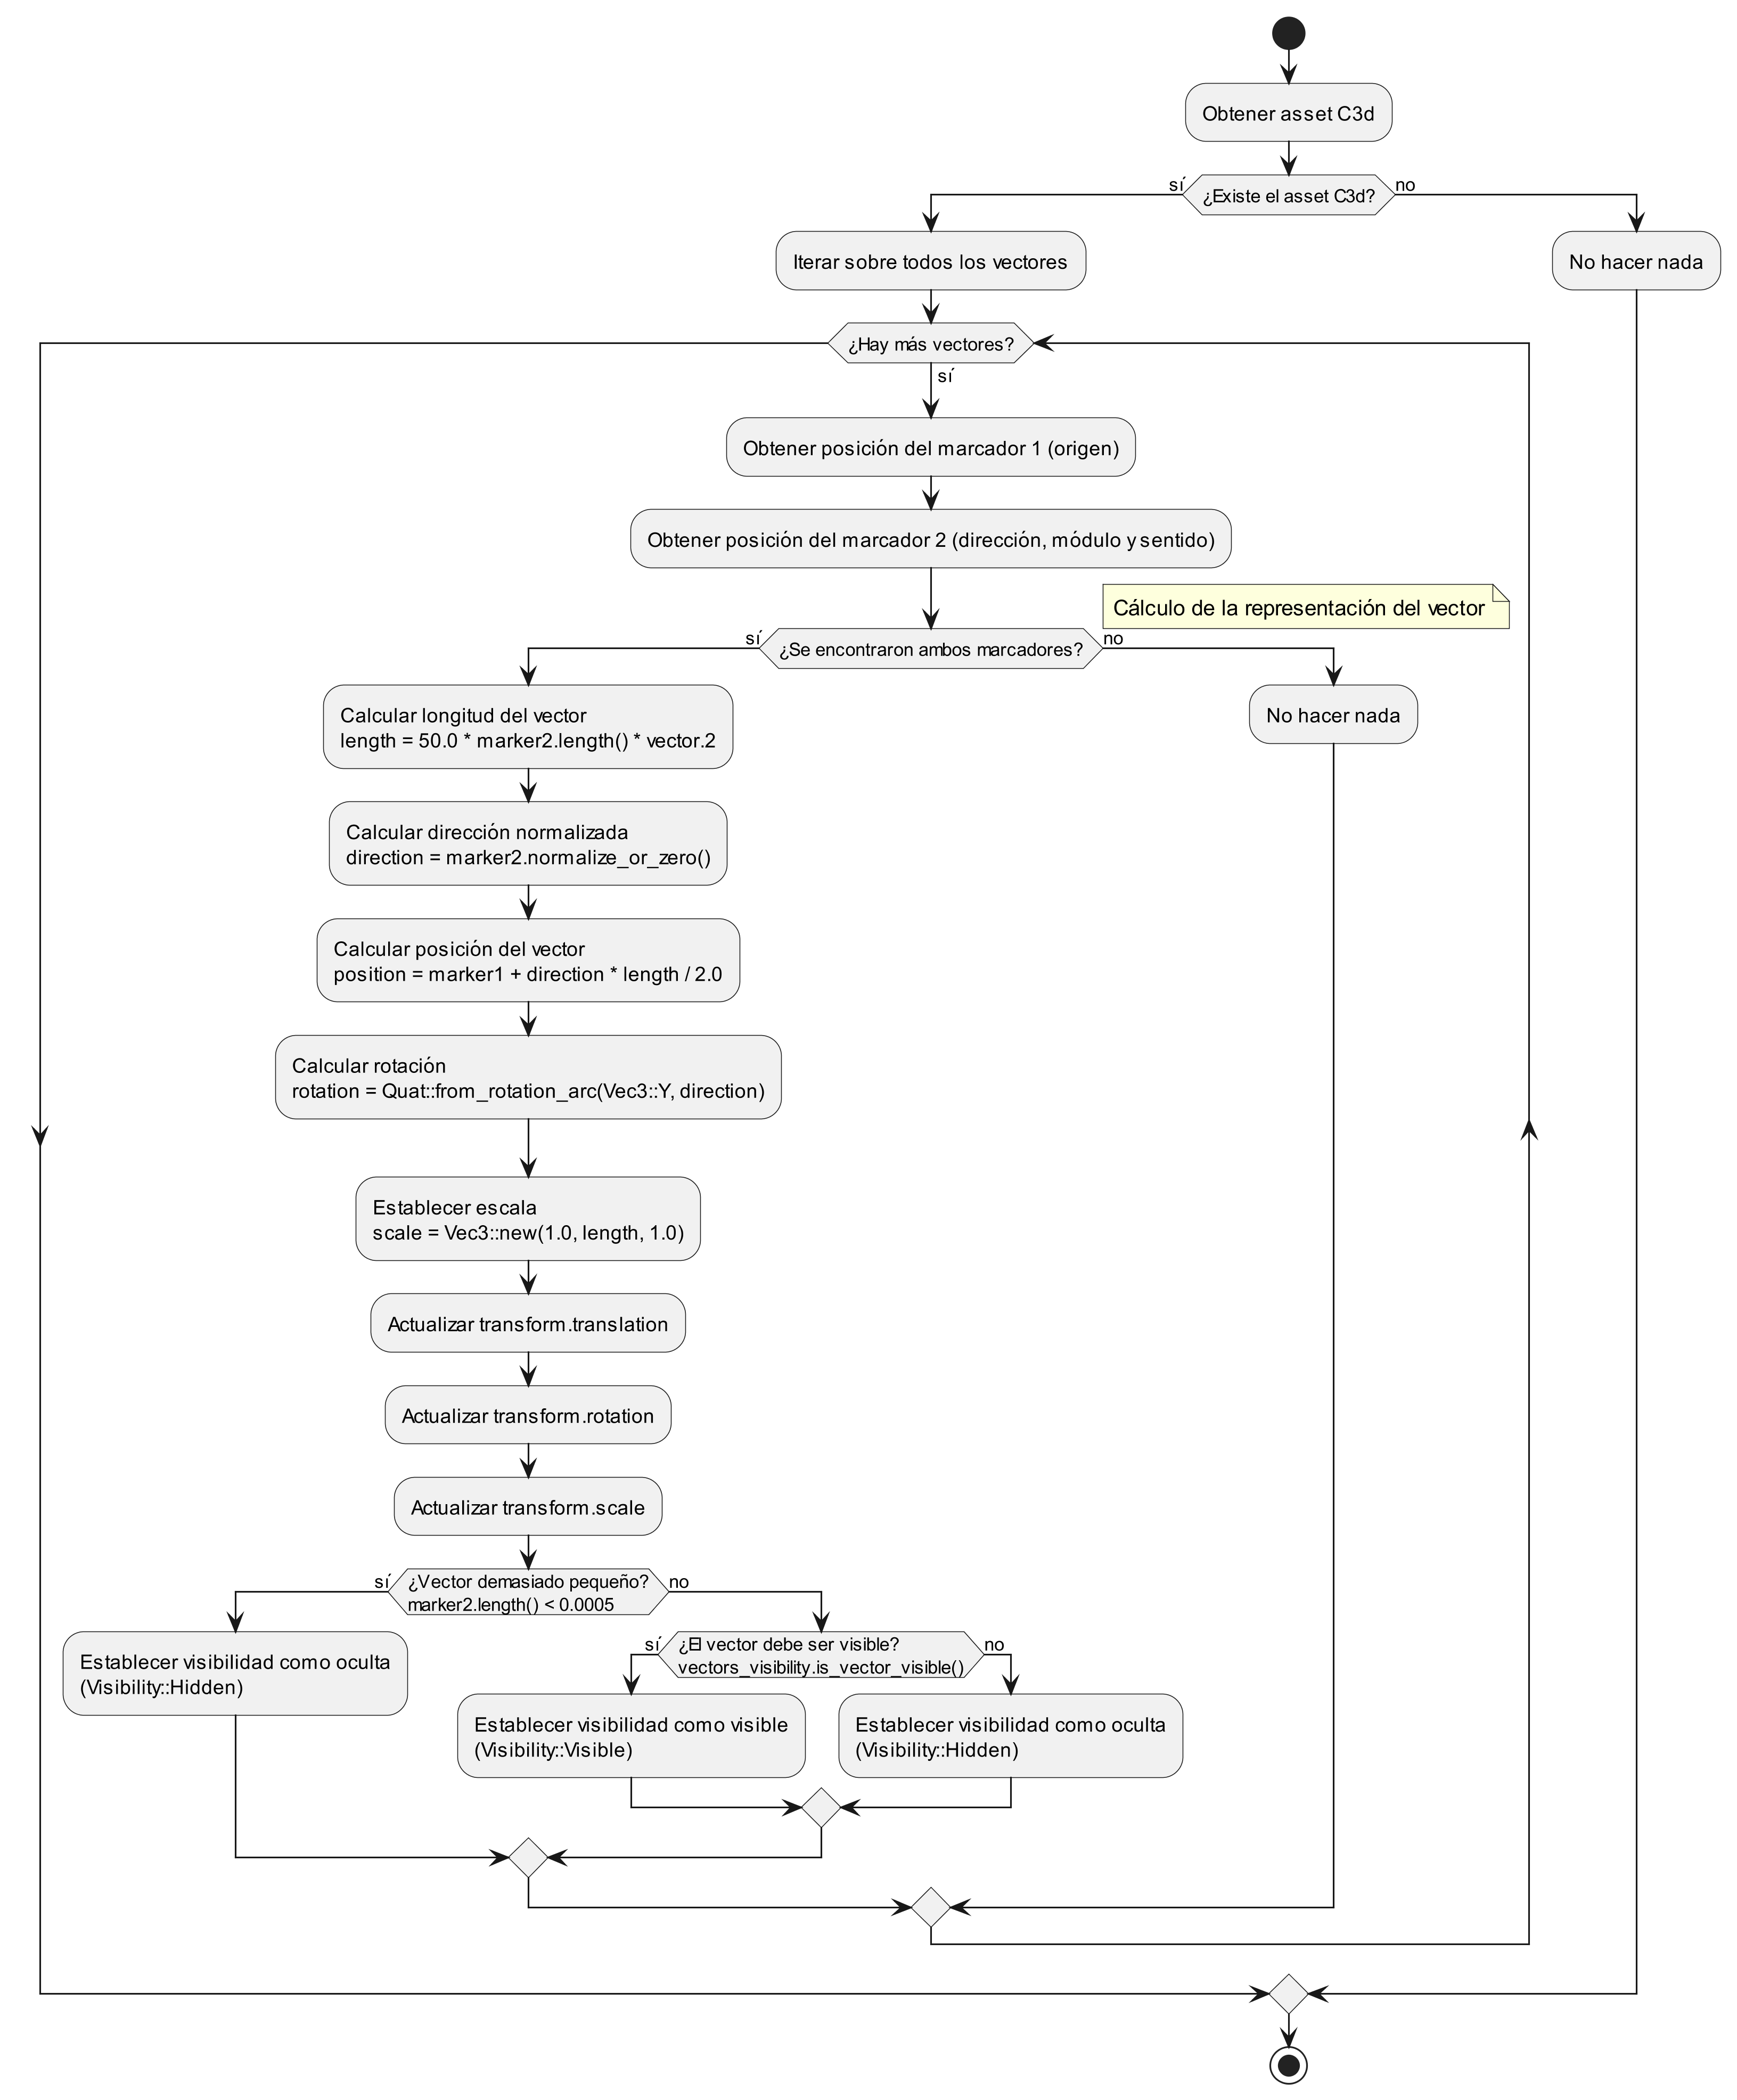
\includegraphics[width=\textwidth]{imagenes/diagramas/vectores.png}
  \caption{Diagrama de actividad sobre la representación de vectores}
  \label{fig:diag-vectores}
\end{figure}

\subsection{Representación de trazas} \label{sec:representacion-trazas}

Las trazas son una representación de la trayectoria de un marcador en el espacio tridimensional. Estas trazas se generan a partir de los fotogramas del \ac{C3D}, y se representan como esferas que eliminan la componente temporal. Es decir, se genera una esfera por cada fotograma y por cada marcador del que se quiere representar la traza, en un rango determinado por el doble \textit{slider} del panel inferior. 

Las trazas en combinación con los vectores ilustran características básicas de la geometría, por ejemplo, si se representa la traza de un marcador y su vector de velocidad lineal, se puede observar que el vector de velocidad es tangente a la traza en cualquier punto. Además, en los puntos donde las esferas están más separadas, el módulo del vector de velocidad es mayor.

En la \autoref{fig:trazas} se muestra un ejemplo de la representación de las trazas de un marcador. En este caso, se han representado las trazas del marcador \texttt{OBJ2}, y su vector de velocidad \texttt{LVelOBJ2}. Se puede observar que el vector de velocidad es tangente a la traza en el punto donde se encuentra la esfera.

\begin{figure}[H]
  \centering
  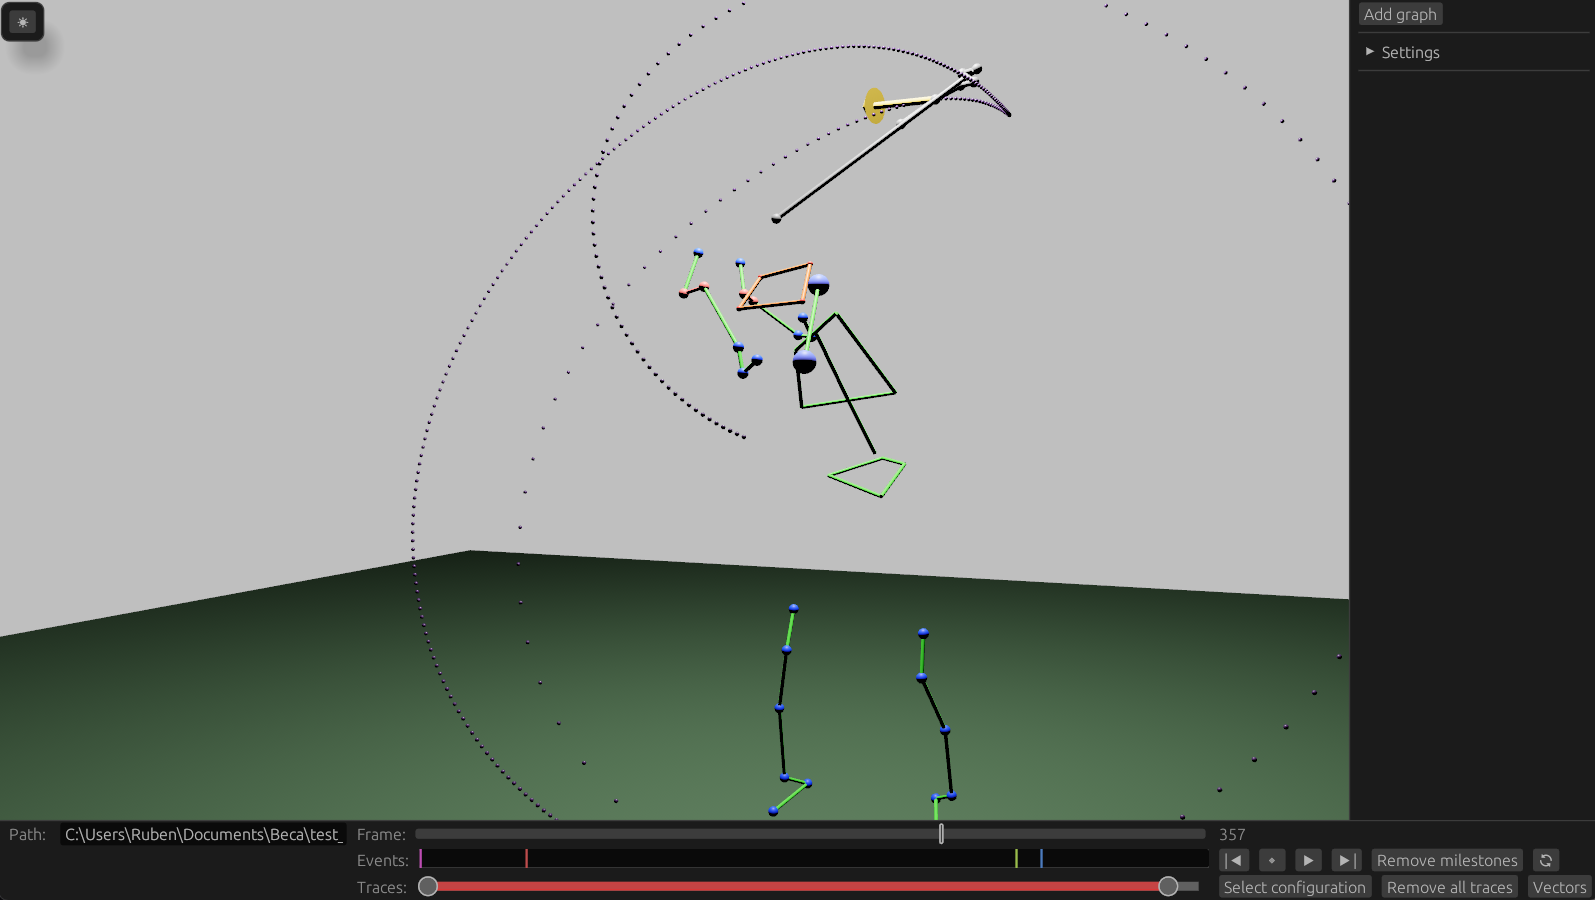
\includegraphics[width=\textwidth]{imagenes/trazas.png}
  \caption{Representación de las trazas de \texttt{OBJ2}}
  \label{fig:trazas}
\end{figure}

Se puede incluir una traza por cada marcador del \ac{C3D}. Todas las trazas comparten el mismo color y tamaño, y el mismo rango de fotogramas, que se puede variar mediante el \textit{slider} del panel inferior. 

Se debe tener en cuenta que generar una traza es una operación muy costosa en memoria y en cómputo, pues se debe recorrer el \ac{C3D} capturando el punto de interés, almacenar su valor en todos los fotogramas y generar un objeto por cada uno de estos puntos. Además, incluir demasiadas trazas suele ser contraproducente, pues genera una cantidad importante de ruido visual.

\subsection{Velocidad de reproducción} \label{sec:modos-reproduccion}

El programa admite dos modos de funcionamiento, velocidad fija o velocidad adaptativa. 

El primer modo es ideal para el estudio de un movimiento con la mayor precisión, esto es, representando la velocidad real de la captura del movimiento, utilizando la tasa de refresco del \ac{C3D}. En caso de que la tasa de refresco de la pantalla sea inferior a la tasa de refresco del \ac{C3D}, \textit{Bevy} realiza una interpolación para que la velocidad de reproducción sea la del \ac{C3D}. Por ejemplo, para una tasa de refresco de una pantalla de 60 \ac{Hz} representando un movimiento de 240 \ac{Hz}, \textit{Bevy} representará uno de cada cuatro fotogramas del \ac{C3D}. Además, este modo permite variar la velocidad de reproducción, entre 0.1 y 2.0 veces la tasa de refresco del \ac{C3D}. 

Por el contrario, el segundo modo es ideal para el estudio del movimiento con la mayor calidad, es decir, sin perder información sobre los fotogramas. En este modo, no se tiene en cuenta la tasa de refresco del \ac{C3D}, \textit{Bevy} representará el fichero respetando las limitaciones del \textit{hardware}. Esto es, si se dispone de una pantalla de 60 \ac{Hz}, como máximo el programa se actualizará a esta velocidad (aunque si hay un componente más restrictivo, por ejemplo una tarjeta gráfica incapaz de dar una tasa de refresco adecuada, se respetará esta limitación). 

En el \autoref{apx:keyboard-shortcut} se muestra una tabla con los atajos de teclado para cambiar entre estos modos.

\section{Interfaz gráfica de usuario} \label{sec:gui}
La interfaz gráfica de usuario se ha desarrollado utilizando el \textit{crate} \texttt{bevy\_egui}, que permite crear interfaces gráficas de usuario en \textit{Bevy} utilizando la biblioteca \textit{Egui}. Esta biblioteca es compatible con \textit{WebAssembly}.

La \ac{GUI} se divide en dos paneles principales, el panel inferior, dedicado al desplazamiento temporal, y el panel derecho, dedicado a la obtención de gráficas de los marcadores, para el análisis de los movimientos. 

\subsection{Panel inferior} \label{sec:panel-inferior}

El panel inferior de la pantalla está mayormente dedicado a la representación temporal del \ac{C3D}. La \autoref{fig:panel_inferior} muestra el panel inferior, focalizando en la parte de la representación temporal. Además de lo mostrado en esta imagen, existe un espacio reservado para representar la ruta del fichero \ac{C3D}.

\begin{figure}[H]
  \centering
  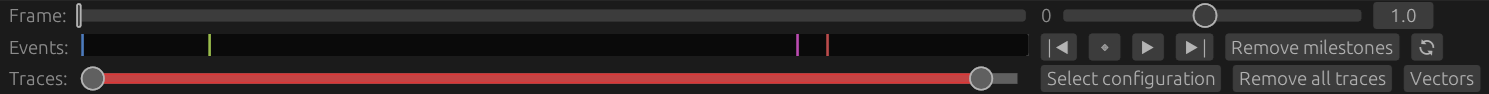
\includegraphics[width=\textwidth]{imagenes/panel_inf.png}
  \caption{Panel inferior de la representación temporal del \acs{C3D}}
  \label{fig:panel_inferior}
\end{figure}


Se distinguen tres filas. En la fila superior, en la parte izquierda aparece el \textit{frame} actual, representado mediante un \textit{slider}, que se puede mover para variar el \textit{frame}, y un número, ubicado justo a su derecha. Adicionalmente, a la derecha aparece otro \textit{slider} que permite ajustar la velocidad de reproducción del \ac{C3D}. Este \textit{slider} solo aparece si se ha seleccionado el modo de velocidad fija, como se explica en la \autoref{sec:modos-reproduccion}.

La segunda fila está dedicada a los eventos del \ac{C3D} (no confundir con los eventos de \textit{Bevy}), que son un parámetro dentro del fichero \ac{C3D} que permite fijar momentos importantes en el tiempo. Los eventos se pueden utilizar para navegar a través de estos momentos clave gracias a los botones de la parte derecha, que de izquierda a derecha significan: retroceder al evento anterior, marcar el \textit{frame} actual como un evento, variar entre pausa y reproducción, avanzar al evento siguiente, eliminar eventos y eliminar los eventos marcados por el usuario, dejando solo los eventos originales del \ac{C3D}.

Para diferenciar los eventos de \textit{Bevy} y los eventos del \ac{C3D}, se ha renombrado a estos últimos como \textit{milestones} (\textit{hitos}).

La última fila contiene un \textit{slider} que permite variar el rango de las trazas, variar entre configuraciones y ver u ocultar vectores. Cuando se pulsa cualquiera de los botones con texto, se abre un menú desplegable que permite seleccionar la configuración deseada.

\subsection{Panel derecho} \label{sec:panel-derecho}
El panel derecho de la pantalla está dedicado a la representación gráfica de coordenadas de posición (x, y o z) de los marcadores a lo largo del tiempo. Dispone inicialmente de un botón que permite añadir un nuevo gráfico, y un desplegable con la configuración global de todos los gráficos. Este desplegable permite cambiar el eje X de los gráficos, teniendo opciones para representación temporal respecto al inicio de la captura, en unidades de segundo, o en unidades de fotogramas.

La \autoref{fig:panel_derecho} muestra el panel derecho en su estado inicial, donde no se ha añadido ningún gráfico. 

\begin{figure}[H]
  \centering
  
\includegraphics[width=0.3\textwidth]{imagenes/panel-dcho.png}
  \caption{Panel derecho de la representación de gráficas de los marcadores}
  \label{fig:panel_derecho}
\end{figure}

Cuando se pulsa el botón de añadir gráfico, se genera una ventana emergente con información sobre todos los marcadores. Esta ventana agrupa los marcadores según la configuración en la que aparezcan, y permite añadir un gráfico por cada componente del marcador. Además, permite añadir trazas, como se puede ver en la \autoref{fig:marker_window}. En esta ventana, los marcadores se muestran en orden alfabético para facilitar la búsqueda. Esta ventana se puede minimizar o cerrar, y se puede volver a abrir en cualquier momento. 

\begin{figure}[H]
  \centering
  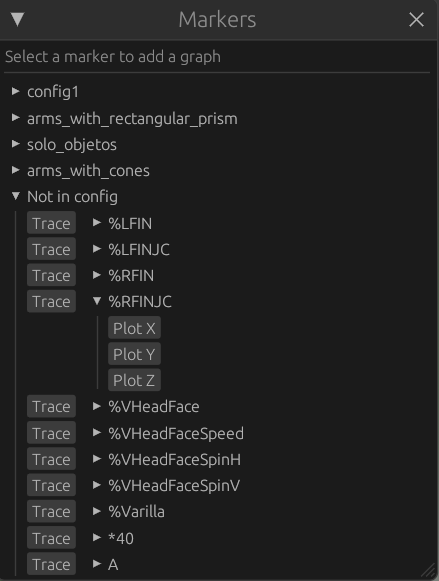
\includegraphics[width=0.3\textwidth]{imagenes/markers-window.png}
  \caption{Ventana emergente con información de los marcadores}
  \label{fig:marker_window}
\end{figure}

La representación de cada una de las componentes es una proyección en 2D, donde el eje X es el tiempo, y el eje Y es la componente del marcador, cuyo significado y unidades dependerá del marcador específico que se represente. Por ejemplo, si se trata de una posición, el valor de la componente Y de la gráfica tendrá unidades de milímetros (e indicará la posición en el eje que se esté representando), y si se trata de una velocidad, tendrá unidades de metros por segundo. Estos gráficos sirven para el estudio del movimiento, y en cada uno se representa el valor de la componente Y de la gráfica en la parte superior derecha.

Cuando se añade un gráfico, este se añade al panel derecho, en la posición que le corresponda siguiendo el orden alfabético, y se puede redimensionar. 
Además, se puede eliminar el gráfico pulsando el botón de eliminar gráfico, que aparece en la parte superior derecha del gráfico. En la \autoref{fig:panel_dcho_con_graficos} se muestra un ejemplo de la representación de gráficos, donde se han añadido los gráficos de las componentes X, Y y Z del marcador \texttt{OBJ1}. 

\begin{figure}[H]
  \centering
  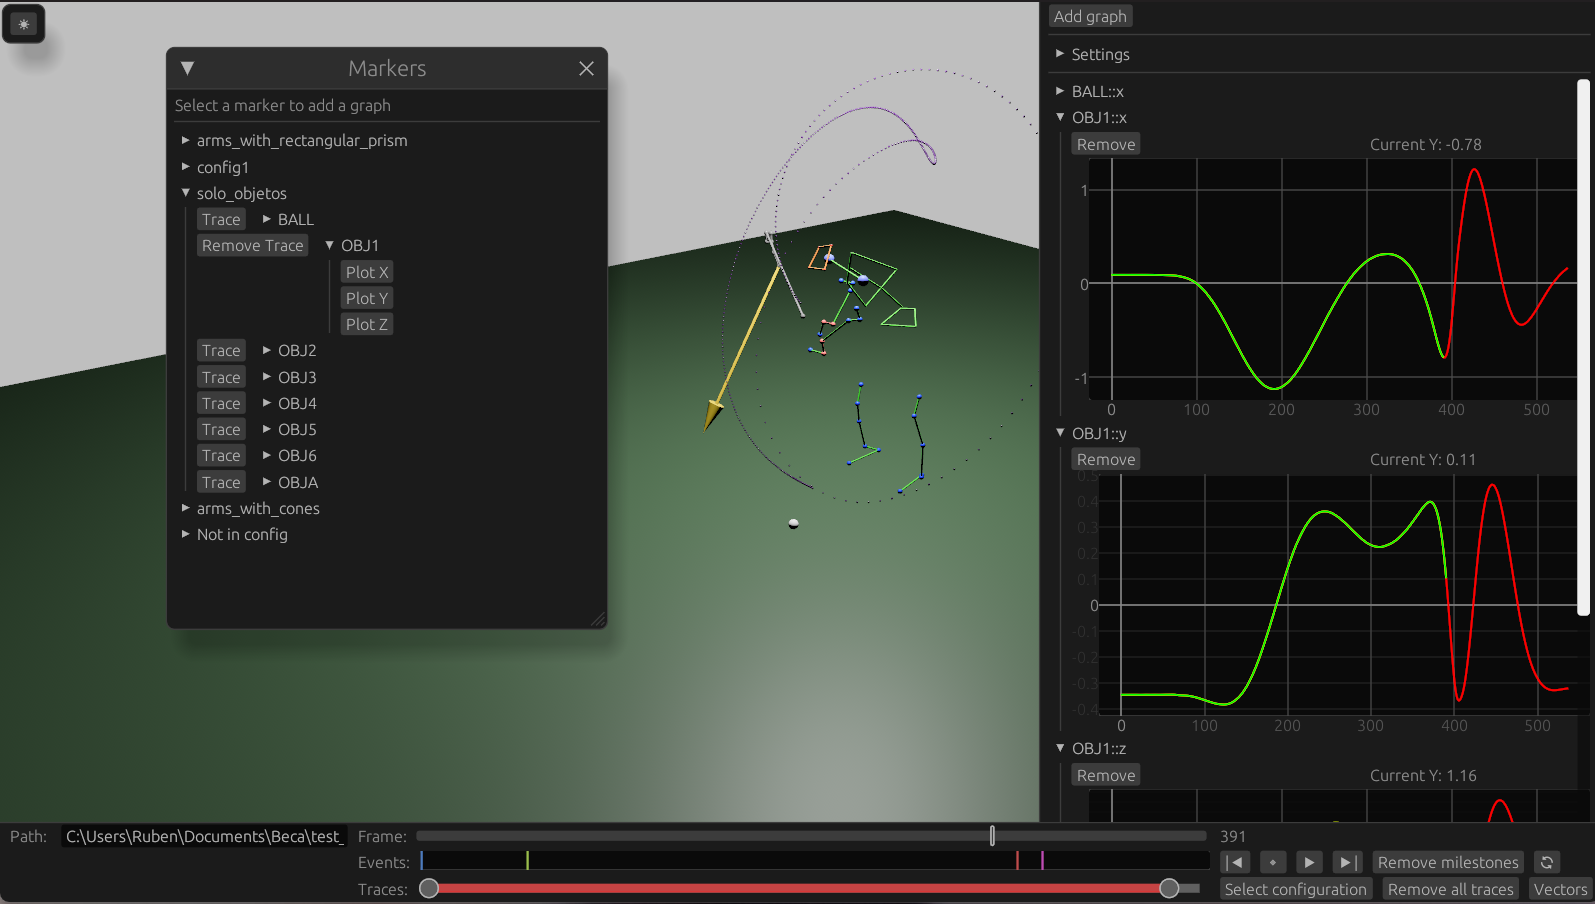
\includegraphics[width=\textwidth]{imagenes/graficos.png}
  \caption{Representación de gráficos en la \acs{GUI}}
  \label{fig:panel_dcho_con_graficos}
\end{figure}

A modo de ejemplo, se incluye la \autoref{fig:estudio_posicion}, donde se hace énfasis en un momento donde un jugador de golf está realizando un movimiento de golpeo.

\begin{figure}[H]
  \centering
  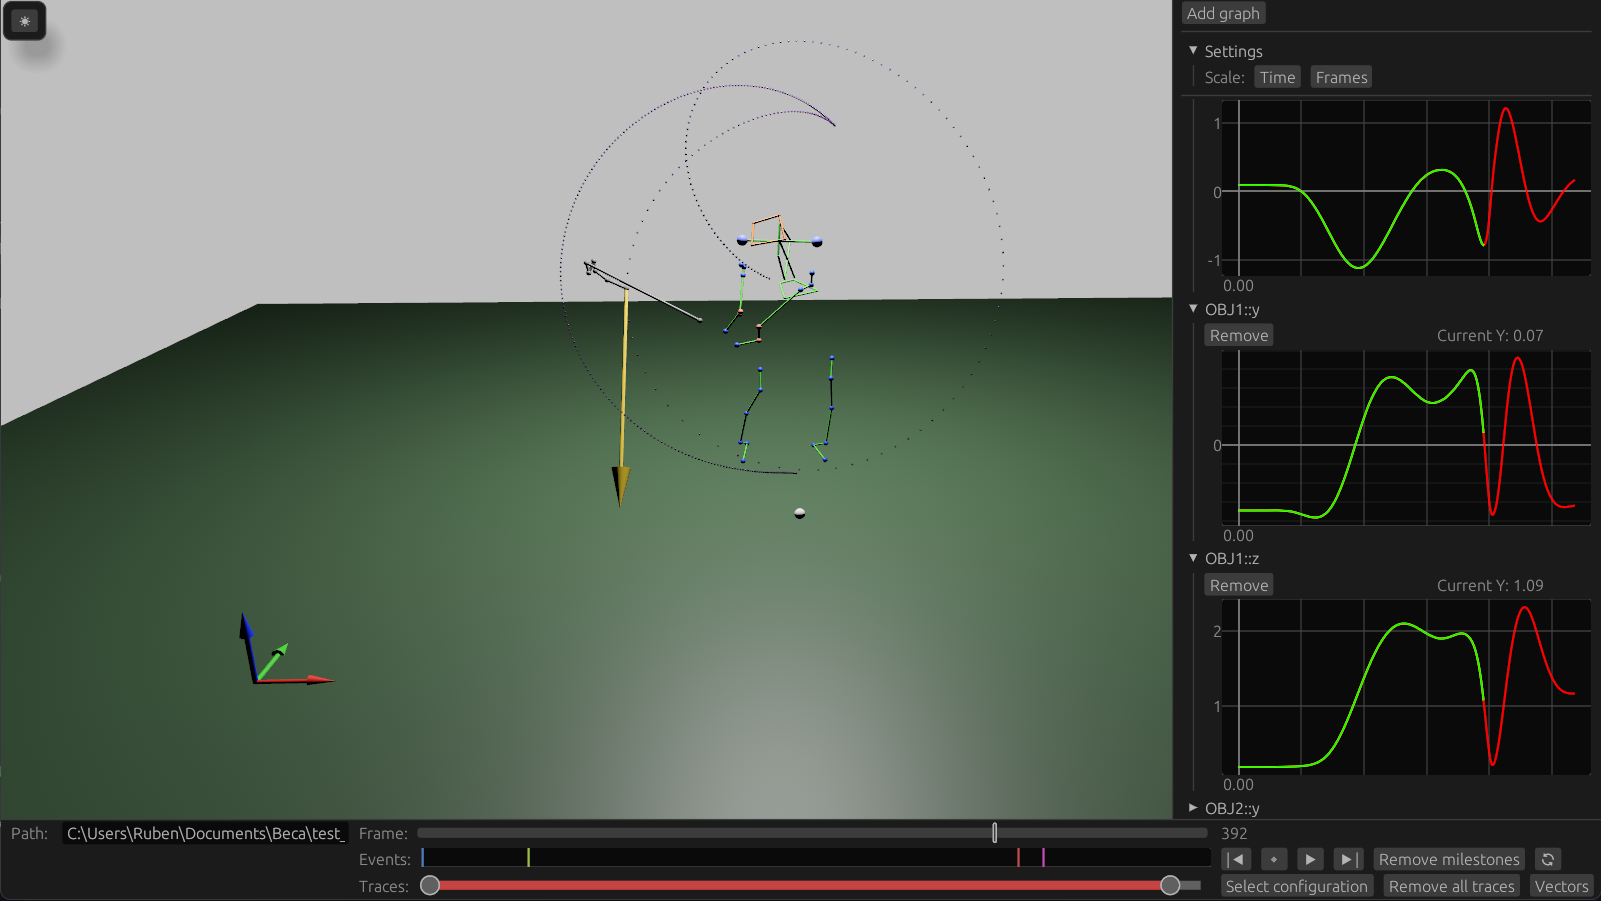
\includegraphics[width=\textwidth]{imagenes/estudio_posicion.png}
  \caption{Estudio de un movimiento}
  \label{fig:estudio_posicion}
\end{figure}

En este instante, el palo se encuentra en una posición tal que la componente X de la velocidad lineal es cero, y las componentes Y y Z son negativas, con un módulo elevado. Se puede comprobar en los gráficos que la componente X de la posición se encuentra en un mínimo, es decir, en este punto no presenta variación, y las componentes Y y Z se encuentran en un momento de variación muy elevado, es decir, con mucha pendiente.

En las figuras anteriores, se puede observar que en el gráfico se marca el pasado con un color verde, y el futuro con un color rojo. La intersección de ambos indica de forma clara el momento actual. Además, en la \autoref{fig:panel_dcho_con_graficos} se puede observar que el panel derecho ocupa un mayor porcentaje de la pantalla que en la \autoref{fig:estudio_posicion}. Como la primera tiene más espacio, se puede añadir información adicional, como marcas en el eje X para disponer de mayores referencias temporales. 

\subsection{Implementación} \label{sec:implementacion-gui}

Siguiendo el enfoque modular del resto del proyecto, la \ac{GUI} se ha implementado como un \textit{plugin} de \textit{Bevy}, que se puede añadir o eliminar en cualquier momento. Esto permite mantener la \ac{GUI} separada del resto del código, y facilita su mantenimiento y evolución.

La \ac{GUI} se ha implementado utilizando el \textit{crate} \texttt{bevy\_egui}, que permite crear interfaces gráficas de usuario en \textit{Bevy} utilizando la biblioteca \textit{Egui}.  

Al arrancar la aplicación, se carga el \textit{plugin} de la \ac{GUI}, que se encarga de crear la ventana y los paneles. La interacción con el resto del programa se realiza mediante eventos de \textit{Bevy}. 

El panel inferior, denominado \texttt{Timeline}, se divide en tres columnas. 

La primera columna contiene una caja con la ruta del fichero \ac{C3D}. El texto de esta caja no se puede modificar, es solo informativo. Cuando se carga un fichero, se actualiza el texto de esta caja, que en la versión de escritorio es una ruta del sistema de ficheros, mientras que en la versión web es una \textit{Blob URL}. 

La columna central ocupa la mitad del ancho disponible, por ser la principal. A su vez, está dividida en tres filas, donde la primera contiene un \textit{slider} con un estilo modificado, ya que se ha modificado el asa para que sea rectangular, con una proporción de 1:10. La segunda fila está dedicada a los eventos del \ac{C3D} que se representan como líneas verticales a la altura del \textit{frame} donde se encuentran. Estas líneas se han implementado como un gráfico de \texttt{egui\_plot}, que es una librería de gráficos para \textit{Egui}. La tercera fila contiene un \textit{slider} con dos asas, para controlar el rango de fotogramas de las trazas \autocite{hacknusHacknusEgui_double_slider2025}.

Por último, la columna derecha contiene botones de control general. Esta columna también se divide en tres filas. La primera fila muestra el \textit{frame} actual, y, en caso de que el modo de reproducción sea de velocidad fija, un \textit{slider} para controlar la velocidad de reproducción. La segunda fila contiene seis botones, de izquierda a derecha: retroceder al evento anterior, marcar el \textit{frame} actual como un evento, variar entre pausa y reproducción, avanzar al evento siguiente, eliminar eventos y eliminar los eventos marcados por el usuario. Por último, la tercera fila contiene tres botones, que permiten cambiar entre configuraciones del fichero de configuración cargado, eliminar todas las trazas y ver u ocultar los vectores.

El panel derecho, denominado \texttt{MetricsDashboard}, contiene un botón que permite añadir un nuevo gráfico, y un desplegable con la configuración global de todos los gráficos. Cuando se pulsa el botón de añadir gráfico, se genera una ventana emergente que permite añadir nuevos gráficos. Internamente, se almacena una estructura de datos que contiene un mapa con el identificador del gráfico (que coincide con el nombre del marcador y la coordenada), y el gráfico en sí, que está compuesto por dos vectores. El primero de ellos representa todos los puntos de la gráfica (se visualiza en color rojo), y el segundo almacena los puntos que se han representado en el pasado (se visualiza en color verde). También se almacena la escala que el usuario decida usar (tiempo o fotogramas). De este modo, para eliminar un gráfico, tan solo se debe eliminar del mapa.

Esta configuración admite tantos gráficos como componentes de marcadores en el \ac{C3D} (tres veces el numero de marcadores). Por tanto, para poder navegar entre gráficos, el panel derecho es un panel deslizante, que se puede desplazar hacia arriba y hacia abajo. Además, cada gráfico tiene un botón de eliminar gráfico, que permite eliminar el gráfico de forma sencilla.

El último componente de la \ac{GUI} es un pequeño botón que permite cambiar el color de fondo de la aplicación, alternando entre un modo claro y un modo oscuro. Este botón se encuentra en la parte superior izquierda de la pantalla, y se puede pulsar en cualquier momento. Este botón muestra el símbolo de un sol o una luna, dependiendo del modo de color actual. Este botón no afecta a la representación del \ac{C3D}, solo cambia el color de fondo de la aplicación, y es independiente del resto de la \ac{GUI}. La implementación hace una consulta a \textit{Bevy} sobre las cámaras que se están utilizando, y cambia el color de estas de manera autónoma. 
